% Template file for a standard thesis
\documentclass[11pt]{isuthesis}

\usepackage[pdftex]{graphicx}

% \usepackage[T1]{fontenc} % This changes fonts to type 1 fonts the
% default in this package is type 3

% Standard, old-style thesis
%\usepackage{isutraditional} \chaptertitle
% Old-style, thesis numbering down to subsubsection
% \alternate

\usepackage{rotating}

% Bibliography without numbers or labels
\usepackage{natbib}
% Use the following line if you want square brackets and numbering
% system. Make sure you use "acm" or similar styles with numbering and
% not apa \usepackage[square, numbers]{natbib} \bibliographystyle{acm}
\bibliographystyle{apa}

% Optional Package to add PDF bookmarks and hypertext links
\usepackage[pdftex,hypertexnames=false,linktocpage=true,
breaklinks=true]{hyperref}
\usepackage{bookmark}

\hypersetup{
  colorlinks=true,
  linkcolor=blue,
  anchorcolor=blue,
  citecolor=blue,
  filecolor=blue,
  urlcolor=blue,
  bookmarksnumbered=true,
  pdfview=FitB
}

% The following piece of code removes extra space on the top of each
% chapter that is default of latex report class documents
\usepackage{etoolbox} \makeatletter
\patchcmd{\@makechapterhead}{50\p@}{0pt}{}{}
\patchcmd{\@makeschapterhead}{50\p@}{0pt}{}{}

% using the etoolbox package to patch the sectional units
% commands to ADD VERTICAL SPACE TO THE TOC
% \pretocmd{\chapter}{\addtocontents{toc}{\protect\addvspace{15\p@}}}{}{}
% \pretocmd{\section}{\addtocontents{toc}{\protect\addvspace{5\p@}}}{}{}

\makeatother
%%%%%%%%%%%%%%%%%%%%%%%%%%%%%%%%%%%%%%%%%%%%%%%%%%%%%%%%%%%%%%%%%%%%%%

%%%%%%%%%%%%%%%%%%%%%%%%%%%%%%%%%%%%%%%%%%%%%%%%%%%%%%%%%%%%%%%%%%%%%%
% In order to change space between the Table of contents items go to
% isuthesis.cls line
% \renewcommand{\l@chapter}[2]{\addpenalty{-\@highpenalty}....  change
% \vkip values

%% This is to minimize orphan lines. Might not be possible to entirely
%% remove them
% Method 1 of doing this \widowpenalty10000 \clubpenalty10000
% Method 2 of doing this
\usepackage[all]{nowidow}

\usepackage{float}

%% Set the margins in the whole document
\geometry{letterpaper, left=1in, top=1in, right=1in, bottom=1in,
  includehead=true}

\usepackage{amssymb}
\usepackage[intoc, english]{nomencl}

%%%%%%%%%%%%%%%%%%%%%%%%%%%%%%%%%%%%%%%%%%%%%%%%%%%%%%%%%%%%%%%%%%%%%%
% Custom stuff
% Table
\usepackage{booktabs}
\usepackage{tabularx}

% Math joy
\usepackage{amsmath}
\usepackage{amsfonts}
\usepackage{amssymb}

\DeclareMathOperator{\evsym}{E}
\newcommand\ev[1]{\evsym\left\langle#1\right\rangle}
\DeclareMathOperator{\vsym}{V}
\newcommand\vv[1]{\vsym\left\langle#1\right\rangle}

% Comments
\usepackage[dvipsnames]{xcolor}
\usepackage{soul}
\newcommand{\LD}[1]{\sethlcolor{Apricot}\hl{\textbf{LD:} #1}}
\newcommand{\JN}[1]{\sethlcolor{ProcessBlue}\hl{\textbf{JN:} #1}}
%\newcommand{\OUTLINE}[1]{\sethlcolor{SpringGreen}\hl{OUTLINE: \textit{#1}}}
\newcommand{\OUTLINE}[1]{}
\newcommand{\TODO}[1]{\sethlcolor{Salmon}\hl{\textbf{[TODO]} #1}}

\graphicspath{{figures/}}

\begin{document}

\DeclareGraphicsExtensions{.jpg,.pdf,.mps,.png}

% \begin{singlespace}
\def\@makechapterheada{\vspace*{-2cm}\titlepage} % in order to reduce
% the space between margin and heading in titlepage
% Template Titlepage File
% Please choose appropriate options for Master's thesis, Doctoral
% dissertations, and creative components. Please read the comments to
% make an informed choice

\@makechapterheada\titlepage  % using definition from thesis.tex
                              % reduce the space between margin and
                              % heading in titlepage
\title{The RITAS algorithm: a constructive yield monitor data
  processing algorithm for soil mapping}

\author{Luis Damiano}

%%%%%%%%%%%%%%%%%%%
%% Master of Science options. CC will have a couple of changes
%% mentioned near the end of this file.
\degree{MASTER OF SCIENCE}
\major{Statistics}

% Use the following line for co-majors (usually used with doctoral
% dissertations)
%\comajors{Statistics; Computer Science}{}

\level{master's}
\mprof{Jarad Niemi}
% In case of co majors please comment out the mprof line above and use
% the following two lines of mprofs and cmprofs to defines the two
% co-major profs
%\mprofs{ABC}
%\cmprofs{DEF}

\members{Petru\c{t}a Caragea \\ Bradley Miller \\}
\disclaimertitlepage{The student author, whose presentation of the
scholarship herein was approved by the program of study committee, is
solely responsible for the content of this dissertation/thesis. The
Graduate College will ensure this dissertation/thesis is globally
accessible and will not permit alterations after a degree is
conferred.}

%{The student author and the program of study committee are solely
%responsible for the content of this dissertation/thesis. The Graduate
%College will ensure this dissertation/thesis is globally accessible
%and will not permit alterations after a degree is conferred.}

%%%%%%%%%%%%%%%%%%%%%%%%%%%%
% Doctor of Philosophy options If co-majors select only co-major
% options as described and skip other options like \major, \mprof and
% make sure committee members are appropriately included.

% Add these additional lines for a Doctoral Dissertation
%\degree{DOCTOR OF PHILOSOPHY}
% \major{Human Development and Family Studies (Marriage and Family Therapy)}
% Use the following line for co-majors (usually used with doctoral dissertations)
%\comajors{Statistics; Computer Science}{}
%\level{doctoral}
%\mprof{Susan D. Ross}
%In case of co majors please comment out the mprof line above and use
%the following two lines of mprofs and cmprofs to defines the two
%co-major profs \mprofs{ABC} \cmprofs{DEF}

%\format{dissertation}
%\committee{4}
%\members{Mary Jones \\ Bjork Petersen \\ Sam Anders \\ Harold Jones}
%\disclaimertitlepage{The student author, whose presentation of the
%scholarship herein was approved by the program of study committee, is
%solely responsible for the content of this dissertation/thesis. The
%Graduate College will ensure this dissertation/thesis is globally
%accessible and will not permit alterations after a degree is
%conferred.}

%%%%%%%%%%%%%%
% Creative component: lines to add / remove
% Add these additional lines for a Creative Component
% - also comment out the \maketitle command
%\format{Creative Component}
%\submit{the graduate faculty}

\notice
\maketitle

%%% Local Variables:
%%% mode: latex
%%% TeX-master: "../thesis"
%%% End:


% Optional thesis dedication
\chapter*{DEDICATION}

To those who have helped me, those who presently help me, and those
who will help me grow.

%%% Local Variables:
%%% mode: latex
%%% TeX-master: "../thesis"
%%% End:


% Table of Contents, List of Tables and List of Figures
\pdfbookmark[1]{TABLE OF CONTENTS}{table}
\tableofcontents
%% The line below adds the word "Page" over the page numbers in TOC,
%% LOT, LOF
\addtocontents{toc}{~\hfill\textbf{Page}\par}
\addtocontents{lot}{~\hfill\textbf{Page}\par}
\addtocontents{lof}{~\hfill\textbf{Page}\par}
%%
\addtocontents{toc}{\def\protect\@chapapp{}} \cleardoublepage
%\phantomsection \pagebreak \addcontentsline{toc}{chapter}{LIST OF
%  TABLES} \listoftables \cleardoublepage \phantomsection
\addcontentsline{toc}{chapter}{LIST OF FIGURES} \listoffigures

% Optional Nomenclature
\cleardoublepage \phantomsection
\makenomenclature
\renewcommand{\nomname}{NOMENCLATURE}
%\specialchapt{NOMENCLATURE}

%\mbox{}
\renewcommand\nomgroup[1]{%
  \item[\bfseries
  \ifstrequal{#1}{A}{Physics Constants}{%
  \ifstrequal{#1}{B}{Number Sets}{%
  \ifstrequal{#1}{C}{Other Symbols}{}}}%
]}

\nomenclature[A, 02]{$c$}{Speed of light in a vacuum inertial system}
\nomenclature[A, 03]{$h$}{Plank Constant}
\nomenclature[A, 01]{$g$}{Gravitational Constant}
\nomenclature[B, 03]{$\mathbb{R}$}{Real Numbers}
\nomenclature[B, 02]{$\mathbb{C}$}{Complex Numbers}
\nomenclature[B, 01]{$\mathbb{H}$}{Octonions}
\nomenclature[C]{$V$}{Constant Volume}
\nomenclature[C]{$\rho$}{Friction Index}

\renewcommand{\nompreamble}{The nomenclature for your dissertation or thesis is optional. This list may be placed in
the following places: as the last preliminary page, before the Reference section, or as an Appendix. The heading is bold if other major headings are bold, and the list is in the same font size and style as text. Nomenclature should follow a two-column format with the term in the left
column and its definition or description within the right column.}

\printnomenclature

% The following link has more tweaks, tips and tricks on how to setup nomenclatures: https://www.overleaf.com/learn/latex/Nomenclatures

% Comment out the next line if NOT using chaptertitle
\addtocontents{toc}{\def\protect\@chapapp{CHAPTER\ }}

% Optional Acknowledgements
\cleardoublepage \phantomsection
\specialchapt{ACKNOWLEDGMENTS}

Funding was provided by Iowa State University through the Presidential
Interdisciplinary Research Initiative on C-CHANGE: Science for a
Changing Agriculture, and the Foundation for Food and Agriculture
Research (FFAR). The dataset used to illustrate our work was collected
as part of the Science-Based Trials of Rowcrops Integrated with
Prairie Strips (STRIPS) project, and involved the work of the US Fish
and Wildlife Service Neal Smith National Wildlife Refuge, numerous
technicians and student researchers, and Heartland Cooperative.

%%% Local Variables:
%%% mode: latex
%%% TeX-master: "../thesis"
%%% End:


% Optional thesis abstract
\cleardoublepage \phantomsection
\specialchapt{ABSTRACT}

Yield monitor datasets are known to contain a high percentage of
unreliable records. The current tool set is mostly limited to
observation cleaning procedures based on heuristic or
empirically-motivated statistical rules for extreme value
identification and removal. We propose a constructive algorithm for
handling well-documented yield monitor data artifacts without
resorting to data deletion. The four-step Rectangle creation,
Intersection assignment and Tessellation, Apportioning, and Smoothing
(RITAS) algorithm models sample observations as overlapping,
unequally-shaped, irregularly-sized, time-ordered, areal spatial units
to better replicate the nature of the destructive sampling
process. Positional data is used to create rectangular aerial spatial
units. Time-ordered intersecting area tessellation and harvested mass
apportioning generate regularly -shaped and \mbox{-sized} polygons
partitioning the entire harvested area. Finally, smoothing via a
Gaussian process is used to provide map users with spatial-trend
visualization. The intermediate steps as well as the algorithm output
are illustrated in maize and soybean grain yield maps for five years
of yield monitor data collected at a research agricultural site
located in the US Fish and Wildlife Service Neal Smith National
Wildlife Refuge.

%%% Local Variables:
%%% mode: latex
%%% TeX-master: "../thesis"
%%% End:


%\cleardoublepage \phantomsection

\newpage
\pagenumbering{arabic}

\section{Introduction}

\cite{Miller1988} were the first to employ geostatistics explicitly in
precision agriculture, a discipline that started in 1990 when
agriculture shifted from farm-level to site-specific crop management
\citep{Oliver2010}. Their study, among other things, introduced
geostatistics for mapping patterns in soil phosphorus or potassium via
interpolation. As defined by the \citet{Council1997}, precision
agriculture is a data-centered discipline comprising data acquisition
at an appropriate scale, data interpretation and analysis, and
management response at an appropriate scale and time. The advent of
big data has been impacting this field largely, especially in terms of
data acquisition, interpretation, and analysis. Computer mapping of
yield and soil is one of the main uses of this technology, typically
to help customize crop management across and within fields by
identifying less productive areas at a sub-field scale
\citep{Lowenberg-DeBoer2019}. Yield data are now recorded
automatically for a wide variety of crops including cereal grains,
oilseeds, fiber, forage, biomass, fruits and vegetables. These data
are known to be accurate at a global scale, yet there exist nuances at
a local scale that affect visualization and downstream analysis, and
jeopardizes the credibility and validity of management decisions
downstream.

\cite{Ross2008} is a synoptic work focused on yield estimation from
yield monitor data covering conceptual, modeling, and mechanical
aspects. \cite{Arslan2002} investigates the impact of yield monitor
calibration in yield estimation accuracy. Although not statistical in
nature, agronomical studies provide with insight on the physicalities
of the system whose sampling process we aim at replicating with our
statistical algorithm. Yield monitoring equipment, introduced in the
early 1990s, is a set of typically more than six sensors, antennas,
and devices attached to combine harvesters that altogether calculate
and record grain yield in real time as the machine operator harvests
the productive field. At the end of each cycle, which lasts a
pre-specified number of seconds that can be adjusted dynamically by
the operator, the monitor logs measurements for more than 15 variables
related to geolocation, crop characteristics, and other machine
diagnostics.

Numerous works have established that yield datasets contain a high
percentage of unreliable data and have proposed cleaning procedures
\citep{Blackmore1996, Moore1998, Blackmore1999, Thylen2000, Noack2003,
  Simbahan2004, Ping2005, Sudduth2007, Sudduth2012, Spekken2013,
  Leroux2018, Leroux2019, Vega2019}. Mechanical measurement errors
have been studied in great depth \citep{Arslan1999, Arslan2002,
  Grisso2002, Burks2004, Hemming2005, Fulton2009, Schuster2017}, yet
we could not find model-based data adjustment protocols. Typically,
systematic errors are identified using either heuristics or
statistical rules with acceptable empirical results but limited
probabilistic motivation. With almost unanimous preference for
systematic error detection and removal, we have found little
development of alternative strategies for error correction or
integration such as the one proposed by \cite{Bachmaier2007,
  Bachmaier2010}; in fact, some methodologies discard as much as one
third of the original dataset as summarized by \cite{Lyle2013}.

In many cases, these procedures require the map user to set values for
tuning parameters such as thresholds. These constants are not learned
from the data but set arbitrarily by the user instead, hindering
comparisons across users, locations, and years. Moreover, manually-set
thresholds become a hurdle in the context of big data: both the amount
and the heterogeneity of yield monitor datasets have been increasing
as raw data become more abundant and diverse. Additionally, there is a
general preference for working with crop yield as the main input of
the cleaning procedures. Being a quantity fusing data collected from
more than one sensor, each with its own propagating measurement error,
it typically has a lower signal-to-noise ratio than the mass random
variable. Also, scaling mass to homogenize unequally-sized
observational units likely potentiates extreme values resulting in a
new variable with higher volatility.

Some processing rules, for example those based on the marginal
distribution of yield, do not consider the spatial nature of the
data. Others collapse all the information in one point on a
2-dimensional plane, thus failing to recognize that the recorded data
are in fact associated with overlapping, unequally-shaped, and
irregularly-sized aerial units. Each observation is in reality a
realization from a continuous spatial stochastic process: time
order and spatial superposition are intrinsic characteristics of the
destructive sampling scheme worth modeling.

The many variables logged by the yield monitor equipment include
harvested mass, geocordinates, distance traveled, and swath width,
which can be used to create an aerial representation of the
data. Depending on the hardware, the reported travel distance and
speed may be measured by a speed sensor, a GPS receiver, a radar, or a
ultranosic sensor \citep{Mulla2013}. When distance is not available,
it can be linearly estimated using speed and cycle length or
approximated using the euclidean distance between two subsequent
coordinates. The swath width, also known as gathering or cutting
width, can be time dependent and the combine's path that may not be
correctly reflected in the data logged by the monitor
\citep{Ross2008}. Although equipments provides the operator with tools
to adjust the effective width dynamically, in many situations the
operator is unable to attend to manual adjustments in real time and
thus the logged values simply represents the maximum width. We have
found three main strategies that have been introduced so far that
combine distance and width to reproduce an approximate spatial
representation.

\cite{Blackmore1999} observed that there is a discrepancy between the
theoretical and the effective harvested area. One of the reasons is
that the recorded header width differs from the width of the header
that is truly full of crop. While in practice it can be set equal to a
fixed proportion of the cutter bar width, e.g. 95\%, land finishes and
areas close to voids require special treatment as the header could
even be empty. In order to avoid any use of the recorded width, and
circumvent the uncertainty associated with it, the authors introduced
potential mapping. In this technique, the recorded mass of data points
belonging to circular neighbourhoods is aggregated and assigned to a
new spatial point whose location corresponds to the circle
geocenter. The aggregated mass is then spatially re-normalized by the
area of the polygons in the Voronoi diagram formed by these new
points. This approach has two limitations. First, it transforms data
into spatial points and thus incurs in information loss about the
shape and size of the observational aerial units (e.g. \ different
shapes could have the same centroid). Second, an additional gridding
technique needs to be applied to analyze temporal trends in yield maps
\citep{Blackmore2003}, effectively displacing the yield measurements
twice: all the polygon information is first collapsed into a single
point which is displaced afterwards.

Previously, \cite{Han1997} introduced a bitmap approach to determine
the actual combine cut width, compute the effective area size, and
approximate the new centroid of each spatial unit after removing the
area covered by previous observations. To track the covered area at
each time step, the author superposes a regular grid where each cell
functions as a bitmask indicating whether the pixel has been harvested
before or not, hence the name of the methodology. The article does not
show how this methodology performs in the presence of sharp turns,
where overlaps tend to be larger during the pivoting motion, as these
seem to have been removed from the analysis. It is worth noting that,
even after processing, the intermediate spatial representations have
some overlap and skips left unexplained by the author. Again, as
these intermediate spatial representations are collapsed into spatial
points, some information is lost. Furthermore, these new data points
may not be spatially aligned if temporal analysis was pursued
next. Finally, the authors warn that the bitmap initialization process
is more complicated when there exists non-crop features such as
rivers, canals, or roadways.

Expanding on the bitmap concept, \cite{Drummond1999} developed a
method where observational units are represented by polygons
constructed from position and trajectory information. These are
processed in chronological harvest order by Boolean subtraction to
compute the actual harvested area during each time step, effectively
retaining full information about the aerial units. As drawbacks, the
authors mention the potential overestimation at the boundaries as well
as the computational complexity of the algorithm. In the general case,
its complexity is order $O(N^2)$, yet several strategies for specific
cases are discussed there.


%%% Local Variables:
%%% mode: latex
%%% TeX-master: "../thesis"
%%% End:

\chapter{The RITAS algorithm}
\label{sec:ritas}

Our algorithm constructs yield maps through the following steps:
Rectangle creation, Intersection assignment, Tessellation,
Apportioning, and Smoothing (RITAS). The overarching goal of this
process is to mimic the real world harvesting processes. Figure
\ref{fig:closeup} provides an illustration of a subset of these steps.

\begin{figure}[h!]  \centering
  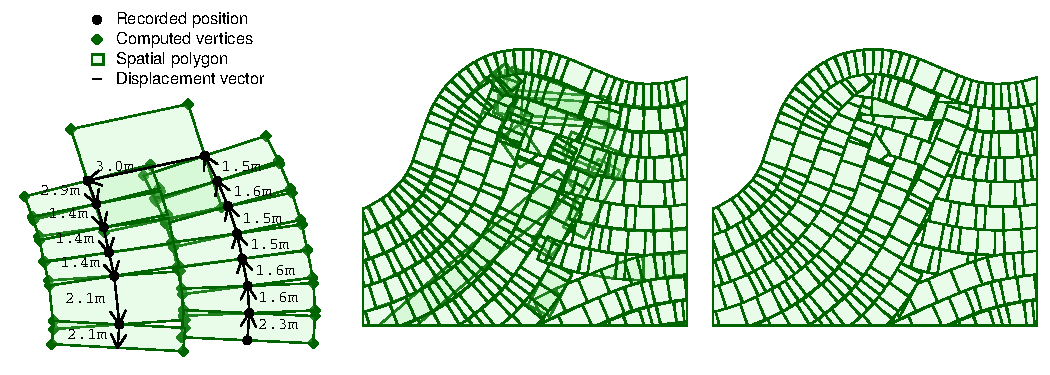
\includegraphics[width=\textwidth]{algoplots}
  \caption[Close-up illustration of selected algorithm steps]{Close-up
    illustration of selected processing steps. \underline{Left}:
    Construction of the vehicle polygons from the GPS location
    data. Black dots mark the location at the end of each logging
    cycle, green dots correspond to the vertices computed according to
    the displacement vector implied by two consecutive spatial
    points. The distance traveled could be reported by the yield
    monitor or estimated from the vector length. \underline{Center}:
    Spatial polygons reveal overlap (darker areas) due to driving
    maneuvers. \underline{Right}: Tessellation eliminates the overlap
    by assigning intersecting areas to the first polygon in time.}
    \label{fig:closeup}
\end{figure}

Each precision yield data set is assumed to have time-ordered rows
containing the following information: mass harvested $m_t$,
2-dimensional spatial coordinate $(x_t,y_t)$, and swath half-width
$w_t$ for $t=0,\ldots,T, \ T \in \mathbb{N}$.  We assume any lag time
has been effectively pre-processed by appropriately matching the mass
harvested to its 2-dimensional location.

\paragraph*{Step 1: Rectangle creation}

Figure \ref{fig:closeup} (left) illustrates the construction of a
rectangular polygon representing the harvested area between each
sequential pair of spatial coordinates. The position vector
$\mathbf{s_t} = (x_{t}, y_{t})$ represents the location of the tracked
device in a 2-dimensional plane at the time step $t$, which we assume
to be the midpoint of the combine harvester head. The rectangle is
then uniquely identified by the position of its four vertices, two
representing the beginning of the harvested area at time step $t-1$
and two representing the end of the harvested area at time step
$t$. The linear displacement vector is equal to the vector difference
between the position vectors at two subsequent time steps
$\mathbf{s_t} - \mathbf{s_{t-1}}$. The first two vertices are computed
as the endpoints of a line segment perpendicular to the displacement
vector with midpoint at $\mathbf{s_{t-1}}$ and length equal to the
swath width $2 w_t$. The remaining two vertices are found using the
same procedure but pivoting on the midpoint $\mathbf{s_t}$
instead. Given a pair of position vectors
$\mathbf{s_t}, \mathbf{s_{t-1}}$, denote
$b_t = (y_t - y_{t-1}) / (x_t - x_{t-1})$ the slope of the connecting
line, and define $dx_t = w_t (1 + b_t^{-2})^{-\frac{1}{2}}$ and
$dy_t = - dx_t b_t^{-1}$. Then, the rectangle associated with mass
$m_t$ has the four vertices coordinates given by
$\{(x_{i} \pm dx_t, y_{i} \pm dy_t): i = t, t-1\}$.

As the first spatial point has no displacement, this processing yields
$T$ rectangles with vertices collected in the set
$\mathcal{P} = \{P_{\tau}$: $\tau \in \{1, \dots, T\}\}$.

\paragraph{Step 2: Intersection assignment and Tessellation}

\OUTLINE{Motivate clipping} Figure \ref{fig:closeup} (middle) shows
end result of this construction which produces rectangles that
overlap, an area called the \emph{intersection}, due to adjacent
harvester paths. Geometries in $\mathcal{P}$ represent the area over
which the combine harvester passed, which may differ from the
effectively harvested area at each time step since the header may not
be full of crop when harvesting the field boundaries (e.g. on outer
edges, around voids), or within them. As a byproduct of the
destructive sampling scheme, the discrepancy is linked to the spatial
superposition of the observational units that arise due to local
harvesting dynamics such as turns, wedges, parallel lines, and
traveling over harvested areas. Globally within a field, this
phenomenon can be exacerbated by factors such as field
characteristics, or narrow row crops \cite{Ross2008}. Generally,
overlapping cannot be assumed symmetrical nor time-invariant. For
example, pivoting motions overlap on the inner side and the proportion
of duplicated area varies at each time step depending on factors such
as the sharpness of the turns, the angle of the wedges, or the
obstacles faced by the operator.

\OUTLINE{Explain clipping} As a general framework to model the
time-varying effectively harvested area, we run a time-ordered
apportioning procedure over the rectangles in $\mathcal{P}$. Let
$\tilde{P}_\tau = P_t \setminus \left( \bigcup_{i = 1}^{t - 1} P_i
\right)$ be the time-ordered relative complement of the previously
harvested area in the rectangle corresponding to the time step $t$. By
doing this, we effectively map the set of overlapping rectangles
$\mathcal{P}$ into a set of non-overlapping polygons
$\tilde{\mathcal{P}} = \{\tilde{P}_{\tau}: \tau \in \{1, \dots, T
\}\}$. When the original dataset has no voids (e.g. unplanted,
flooded, or more generally inaccessible sub areas),
$\tilde{\mathcal{P}}$ form a flat plane covered by tiles with no
overlaps and no gaps (non-periodic tessellation). Some of the
computational considerations discussed in \cite{Drummond1999}, such as
the time scaling and appropriate techniques to reduce algorithm
complexity, are relevant for implementing this step.

This step creates $T$ polygons partitioning the harvested area, each
associated with the same mass it had in Step 1 but now the area may be
smaller (due to the intersection removal) and thus yield is more
accurately captured.

\paragraph*{Step 3: Apportioning} \OUTLINE{Motivate
  gridding \& apportioning} The elements in $\tilde{\mathcal{P}}$ are
unsuitable for spatial techniques that do not accommodate areas with
irregular shapes and heterogeneous area sizes. Two equally-sized long
rectangles, one in a vertical and the other in a horizontal position,
would have the same centroid yet they convey different information
about yield to the north or west of the centroids. Alternatively, two
centered equally-shaped polygons with different sizes carry different
information about the spatial coverage of the collected
data.

To normalize the areal representation in terms of both shape and size,
we superimpose a regular grid of square pixels, assign portions of the
polygons into grid pixels, and apportion the harvested mass associated
with the polygons to the pixels. The first two steps involve topology
operations on geometries whereas the last one involves manipulation of
the numerical data. Accounting for these two spatial features is by
itself a methodological improvement over the surveyed algorithms,
which simply reduce data to spatial points such as the displacement
vector endpoint or, less commonly, the polygon centroid.

\OUTLINE{Explain gridding \& apportioning} Let $\mathcal{P}^{*}$ be
a set of $N \in \mathbb{N}$ equally-sized, non-overlapping, and
contiguous squared pixels forming a partition covering all the
elements in $\tilde{\mathcal{P}}$. The constant $N$ reflects the user
preference in terms of resolution, selected either by the total number
of pixels, more intuitively by the pixel length in meters, or the
target computational time investment. Although pixels size can be set
arbitrarily, its choice should consider the accuracy of the position
system. We take the pairwise intersection among the elements in
$\tilde{\mathcal{P}}$ and $\mathcal{P}^{*}$ and compute
$\pi_{\tau, n} \in [0, 1]$ the proportion of the area in the $\tau$-th
non-overlapping polygon $\tilde{P}_{\tau}$ that intersects with the
$n$-th pixel in the grid for $\tau \in \{1, \dots, T\}$ and
$n \in \{1, \dots, N\}$. The corresponding proportion of the harvested
mass $m_{\tau}$ associated with $\tilde{P}_{\tau}$ is assigned to
$P^{*}_n$. The total harvested mass associated with the $n$-th pixel
is given by $m^{*}_n = \sum_{\tau = 1}^{T} \pi_{\tau, n} \
m_{\tau}$. The resulting polygons in $\mathcal{P}^{*}$ resemble much
the Basic Areal Units (BAUs) as defined by \cite{Nguyen2012} in the
context of massive data fusion: fine-scale, nonoverlapping, areal
regions representing the smallest resolution at which data is
aggregated.

\OUTLINE{Apportioning key fact (1)} Two key aspects behind the
gridding strategy are worth mentioning. First, for the purpose of
apportioning, we assume that the harvested mass associated with the
spatial polygons is distributed uniformly within each unit. This is a
sensible assumption in this context as combine harvester log data in
short cycles and the spatial polygons represent small areas for the
scale of the underlying crop growth process.

\OUTLINE{Apportioning key fact (2)} Second, if one imposes regularity
and equal-shape conditions on the grid elements and also forces it to
cover all the elements in $\tilde{\mathcal{P}}$, the sum of the
pixels area may exceed the sum of the tessellated polygons area. The
excess, found at both the harvested region outer borders and the inner
voids boundaries, can be diagnosed visually with ease. It decreases as
the grid resolution, or equivalently as the total number of pixels
$N$, increases and so can be controlled at the cost of additional
computational time for topology operations and smoothing. %More
Concretely, when a Gaussian Process is applied for smoothing as
described below, exact inference has time complexity in the order of
$O(N^3)$ and storage demands of of $O(N^2)$. In other words, as we
double the map resolution, we octuple the number of operations and
quadruple the need for storage.  Alternatively, one could exclude the
pixels with less than an arbitrary proportion of area effectively
covered by the tessellated observations. A sensible choice, such as a
minimum coverage of 50\%, will tend to balance under and over-covered
polygons. Due care should be taken so that apportioning is still
applied validly: mass should be allocated to pixels only in proportion
of the actual overlapping area, discarding any part of the tessellated
polygons that is not covered by any pixel. Note that the grid
resolution serves only for the purpose of spatial aggregation, and
need not be the same resolution used for the visualization that will
be introduced in the following step.

This step creates $N$ polygons, determined by the user based on
tesselation resolution, partitioning the harvested area each with an
associated mass of harvested crop. Figure
\ref{fig:basswood2012-main-steps} (bottom left) shows the regular grid
with apportioned mass. The regular tesselation provides constant areas
and meaningful centroids, and therefore we can use standard spatial
smoothing techniques directly on mass, as opposed to yield.

\paragraph{Step 4: Smoothing} \cite{McCullagh2006} provided empirical
evidence suggesting that the non-anthropogenic spatial variation in
yield, defined as patterns that cannot be explained by topography or
human intervention, matches the characteristics of the de Wijs process
plus white noise. We smooth using a Gaussian Process (GP) with a
Mat\'ern covariance on the logarithm of mass
\citep{handcock1993bayesian,gutt2006studies}, which becomes similar to
a de Wijs process as the length scale tends to zero. Compared with the
more common powered exponential covariance functions, e.g. Gaussian or
exponential, the Mat\'ern adds an additional parameter that controls
local smoothness, i.e. \ differentiability, and therefore is often
more accurate for real world processes.

Covariance parameters are estimated via Maximum Likelihood, and
smoothed values are found for each tile following \cite{Cressie1993}.
Specifically, for each pixel we have a predicted mean
$\hat\mu_{\ell} \in \mathbb{R}$ and variance
$\hat\sigma^2_{\ell} > 0$ for the logarithm of mass.  We using the
following formulas to convert back to the mean and variance of mass
\[ \hat{\mu}_{m} = \exp\left(\hat{\mu}_{\ell} +
\hat{\sigma}^2_{\ell}/2\right), \quad\mbox{and}\quad
\hat{\sigma}^2_{m} = \exp\left(2 \hat{\mu}_{\ell} +
\hat{\sigma}^2_{\ell}\right)
\left[\exp\left(\hat{\sigma}^2_{\ell}\right) - 1\right].
 \] Finally, yield is calculated by dividing the tile mass by the tile
area.

We have implemented our algorithm in the R programming language, using
the R packages doParallel, foreach, gstat, rgeos, and sp
\citep{Pebesma2004, Pebesma2005, Bivand2013, Graeler2016,
  Microsoft2017, Corporation2018, RCT2019, Bivand2019}.
% Our open-source
% `yieldMaps` package contains routines for the algorithm described in
% the article, visualization routines, and the dataset employed in the
% case study. The algorithm routines were programmed as smaller, modular
% tasks so that users could easily adapt the source code to custom needs
% such as designing a different gridding and aggregation strategy, or
% employing another spatial interpolation model. Visualization routines
% include map generation as well as object movement and polygon creation
% visualizations.

%%% Local Variables:
%%% mode: latex
%%% TeX-master: "../thesis"
%%% End:

\section{STRIPS yield mapping}

\OUTLINE{Introduce section} In this section, we illustrate the
functioning and the results of our methodology when applied to yield
monitor data collected from the same agricultural site over the
years. We start with a detailed discussion of the production of the
yield map for one specific year, and we finally show some resulting
visualizations for the same fields but different crops and years.

\OUTLINE{Introduce data context} The data arises from a study
conducted at the Neal Smith National Wildlife Refuge in central Iowa
to quantify the impact of grassland-to-cropland conversion on
nitrate-nitrogen (NO\textsubscript{3}–N) concentrations in soil and
shallow groundwater and to assess the potential for perennial filter
strips to mitigate increases in NO\textsubscript{3}–N levels
\citep{Zhou2010}. The experiment was run in different study sites
within the 3000-ha area managed by the U.S. National Fish and Wildlife
Service, located in the Walnut Creek watershed in Jasper County,
Iowa. In this case study, we focus on one specific site named Basswood
that is situated west to the Basswood Trailhead.

\OUTLINE{Introduce data specifics} Basswood, located at WGS84 15 N
0477097E 4598644N, has a total area of approximately 13 Ha. Nearly
81\% of the surface is cropland; most of the remaining proportion is
reconstructed prairie vegetation planted as part of the experimental
design. For the purpose of our yield maps, these areas are treated as
voids because no data were collected from that surface. Cropland in the
experiment is in a maize–soybean rotation using standard no-till soil
and weed-management techniques. Geographic coordinates, sample time,
moisture content, and maize (2008, 2010, 2012, 2014) and soybean (2009,
2011, 2013, 2015) flow rate were reported by a Case IH AFS Pro-600
combine-mounted yield monitor every 1-3 s during crop harvest,
resulting in a fine-scale spatially referenced dataset of crop yields
across the study area. \cite{Schulte2017} provides a detailed account
of the experiment protocol and the resulting improvements in the
biodiversity and the delivery of multiple ecosystem services.

\OUTLINE{Describe data} The yield monitor dataset for the year 2012
has 4,239 observations logged each three seconds starting from the
southwest corner of the site. The swath width was reported to be
constant at 6.10 m as the operator did not adjust the proportion of
cut head while driving. The distance traveled during each cycle, with
an overall mean of 3.7 m, has three modes with centers at 1.9, 4.0,
and 6.0 m. The distribution of the yield reported by the monitor, with
its median located at 6.3 mg/ha and the 90\% of observations being
within 1.4 and 10.8 mg/ha, is symmetric and platykurtic. Visual
inspection suggests that there are approximately 20 extreme values on
the right tail. Small areas within the field boundaries without data,
visualized as voids in the maps, correspond to small portions of soil
allocated for nonproductive purposes (e.g. perennial crops, research
equipment).

\begin{figure}[h!]  \centering
  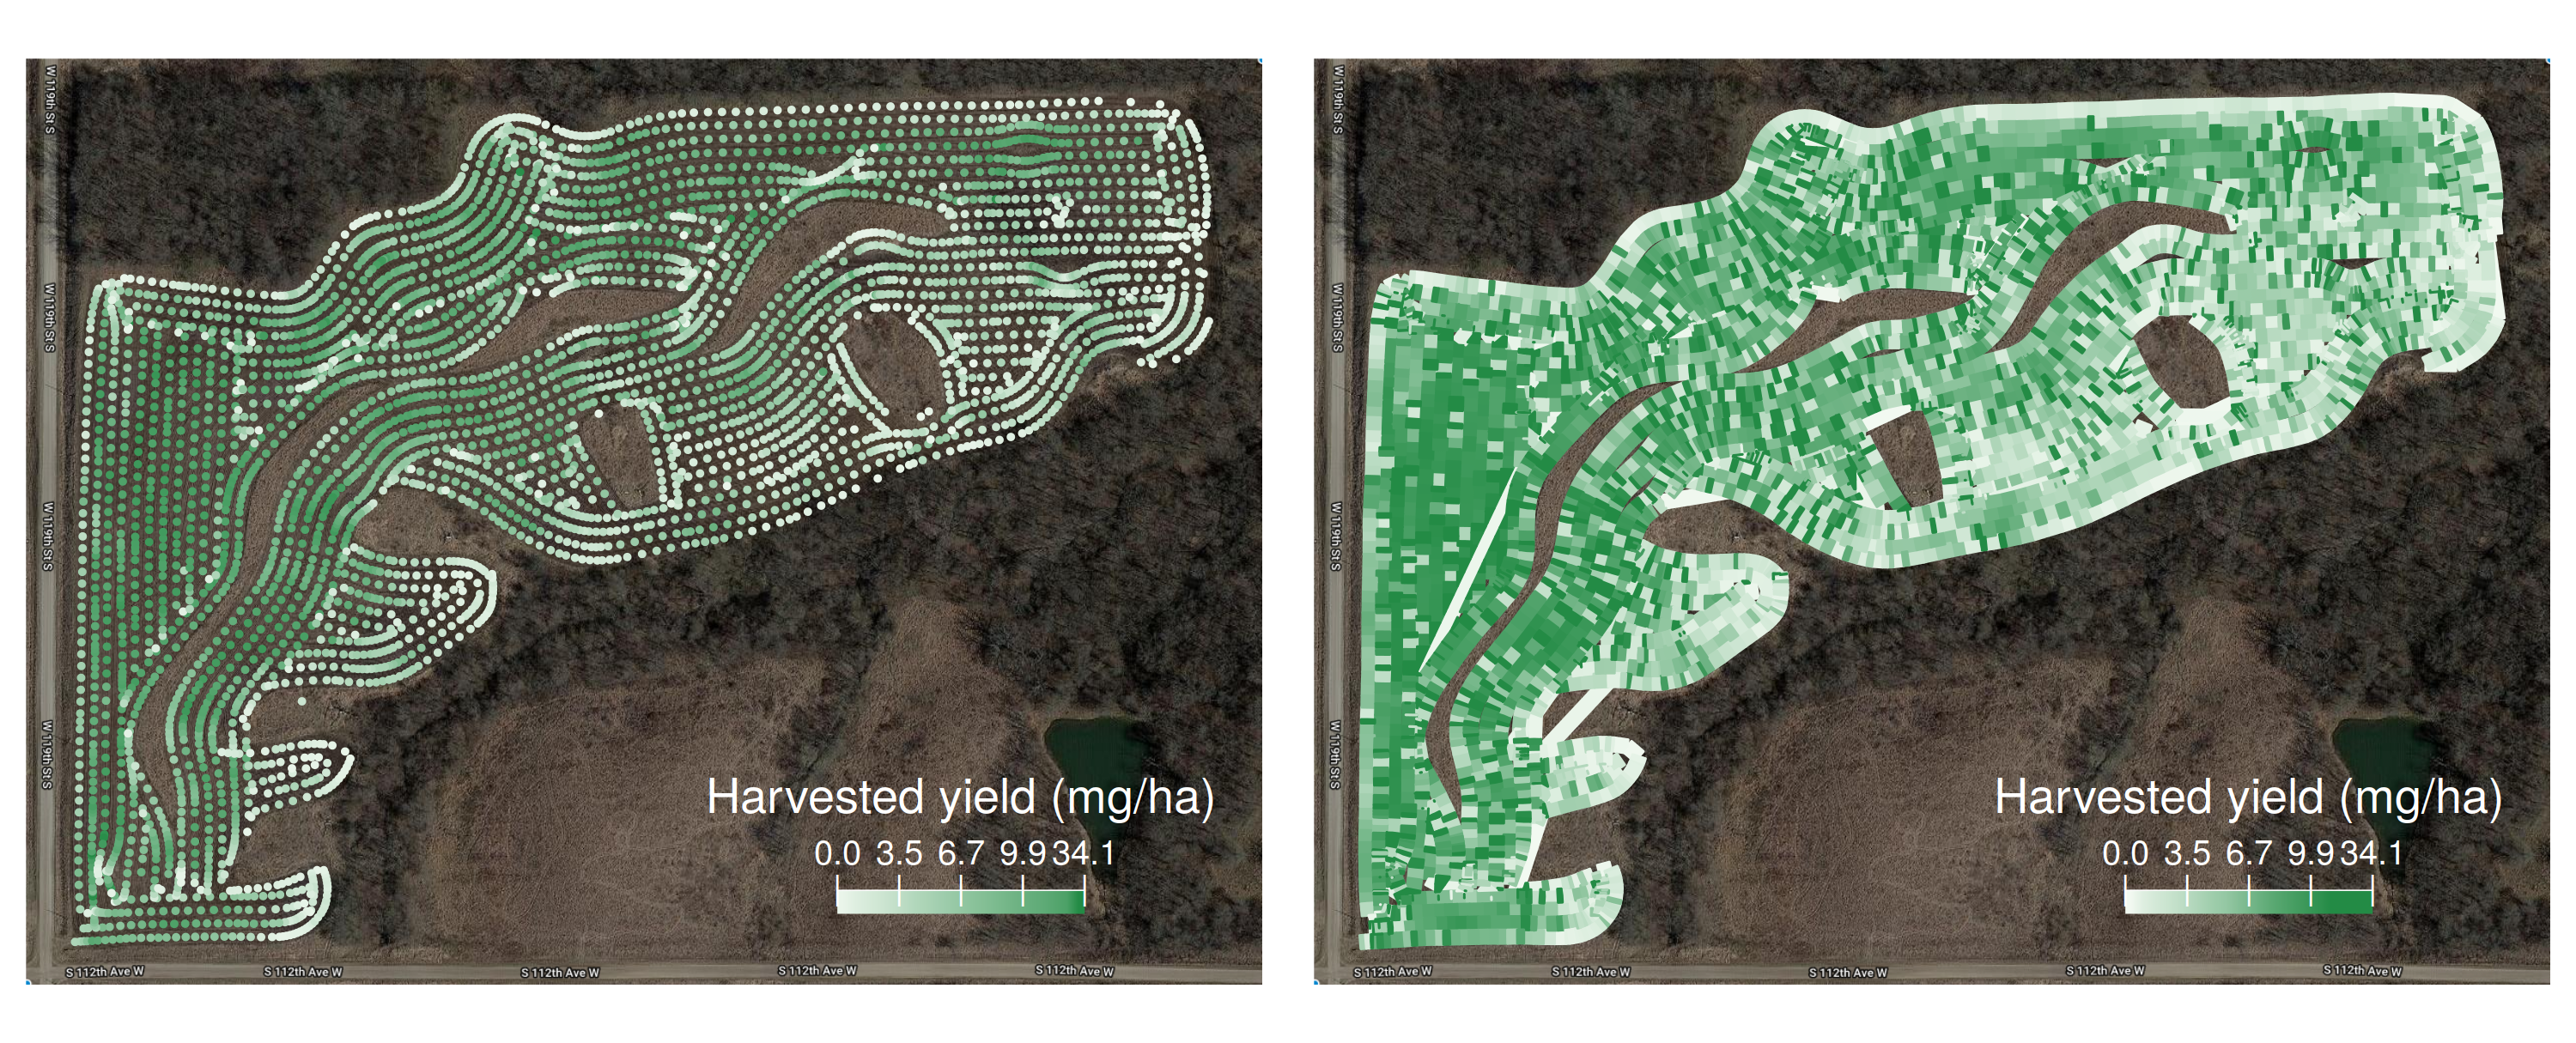
\includegraphics[width=\textwidth]{basswood_2012_res5_points_vehicle}
  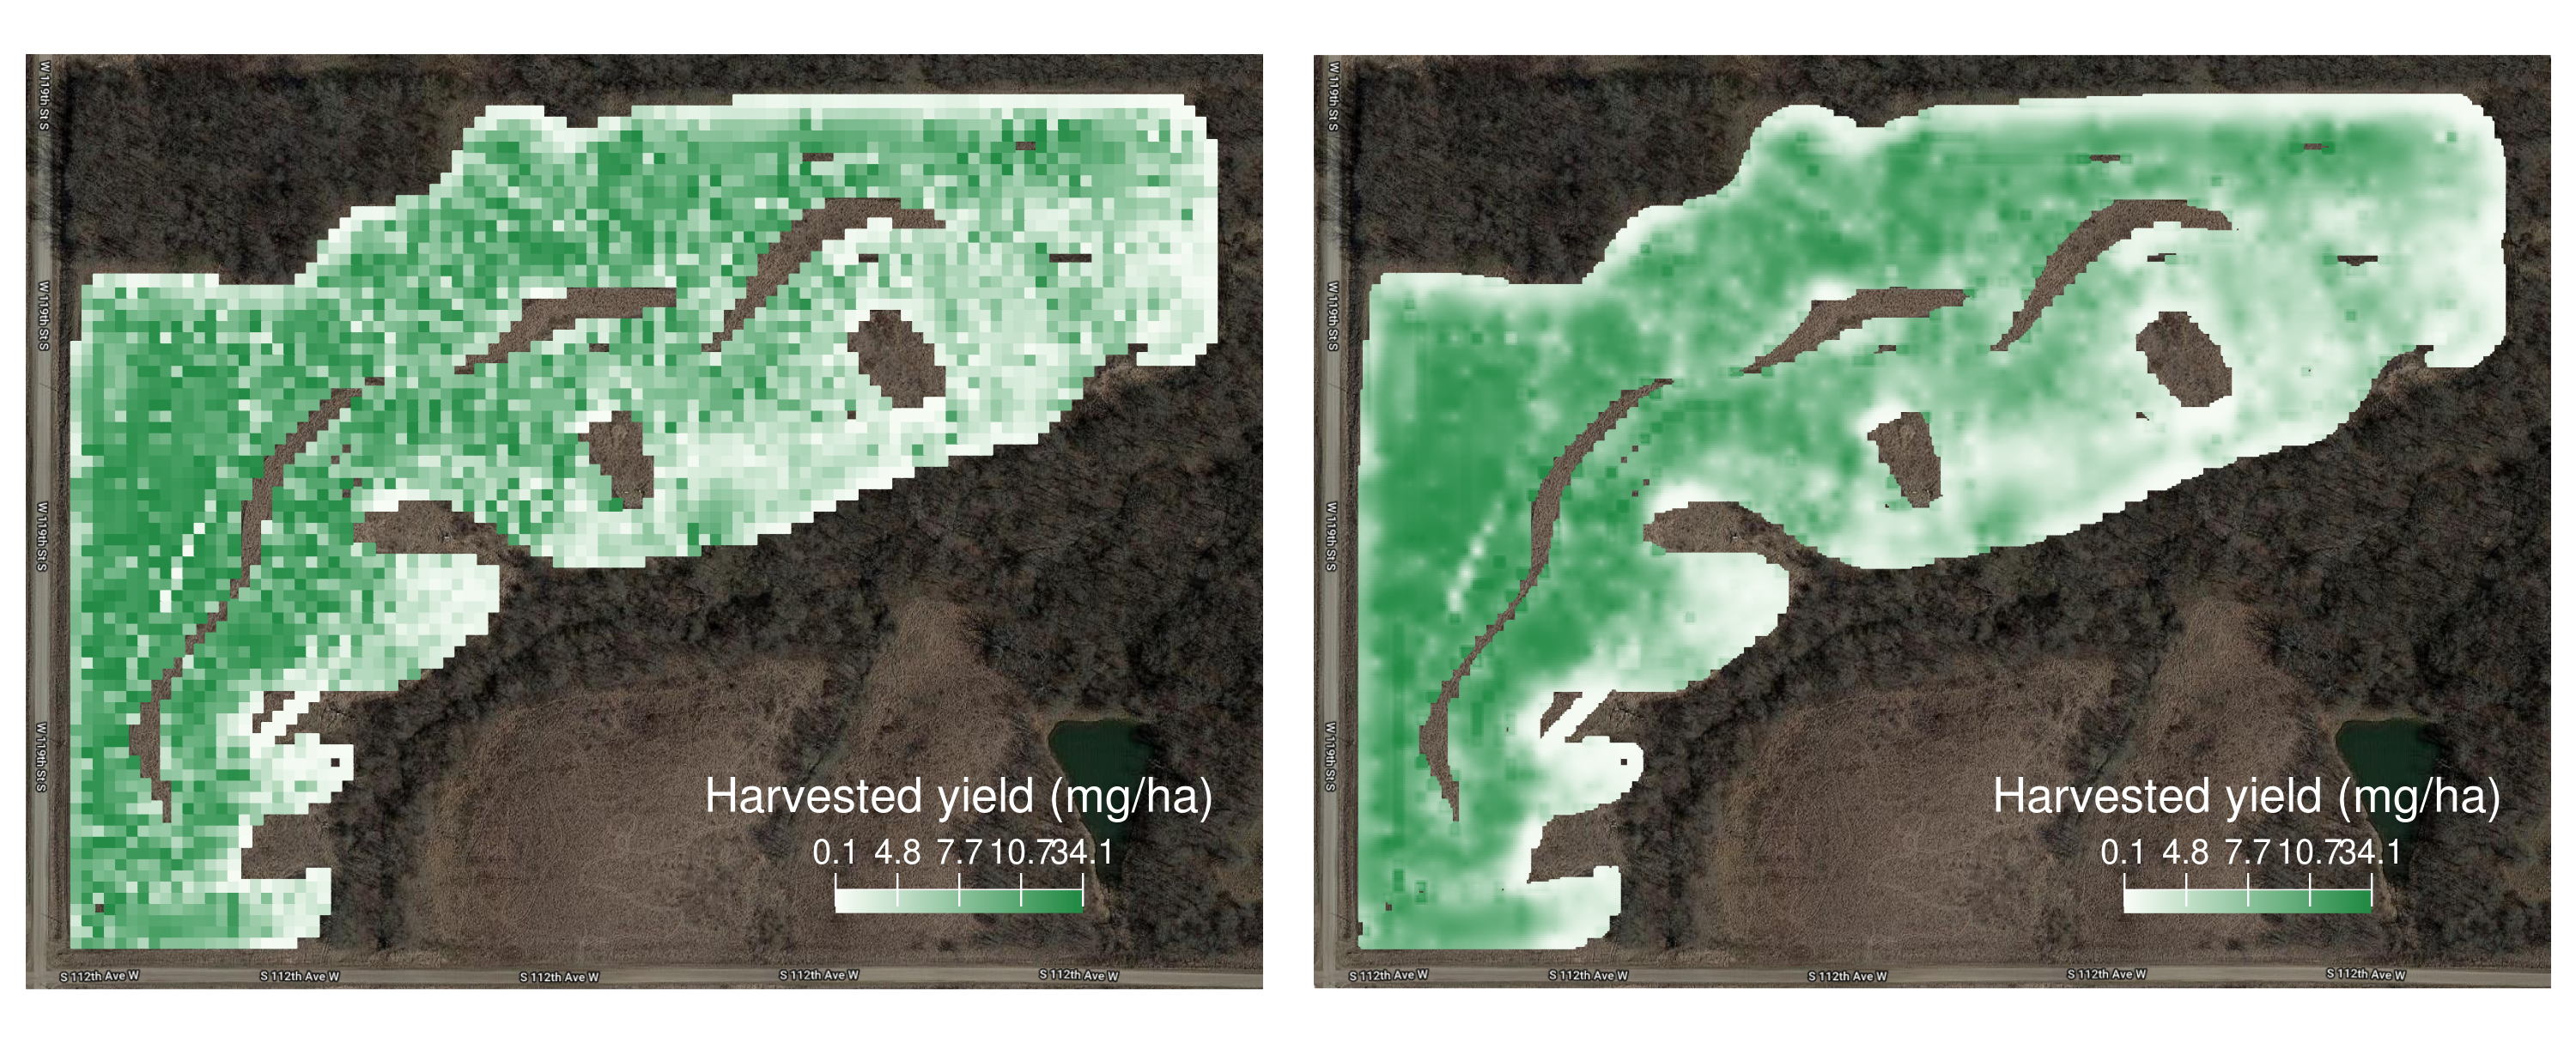
\includegraphics[width=\textwidth]{basswood_2012_res5_1_agg_smoothed}
  \caption[Visualization of selected algorithm steps as applied to a
  specific dataset]{Visualization of selected intermediate steps involved
    in the algorithm for the harvested grain yield of Basswood on year
    2012 (maize). \underline{Top left}: Point map where each observation is
    marked with equally-sized points placed at the each logging
    location. Information relevant to spatial trends are hard to observe,
    such as area coverage and overlaps. \underline{Top right}: Map of the
    clipped polygons. Highly intertiment coloring in noisy areas hinder
    the visualization of the spatial trends, hence the need for
    smoothing. \underline{Bottom left}: Map of the aggregated grid at a 5
    m resolution. This step produces equally-sized, regularly-shaped
    polygons suitable for spatial interpolation. \underline{Bottom right}:
    Map to be shown to the user. By increasing color homogeneity at a
    local level, low and high yield areas have a larger contrast and
    become easier to identify.}
  \label{fig:basswood2012-main-steps}
\end{figure}

\OUTLINE{Introduce dot maps} Figure \ref{fig:basswood2012-main-steps}
(top left) displays the simplest form of a yield map. Data points are
visualized as equally-sized symbols with colors indicating the yield
level at each location. A single-hue shade of green is chosen to ease
the interpretation with dark shades being intuitively associated with
relatively higher crop yield. The characteristics of the yield
distribution vary largely across sites, crop types, and years. Since
the main objective of yield map analysis is to identify sub-field
areas with different performance levels, the points are colored
according to a measure of relative yield within the dataset as opposed
to an absolute scale. As a general rule, we define the color gradient
as a function of the the empirical quartiles in order to guarantee
that low and high yield measurements are uniformly represented at the
same time that the interpretation guidelines remain consistent across
maps.

\OUTLINE{Describe dot map} The proposed coloring scheme helps
capturing the large-scale spatial trends: the east area, both above
and below the perennial crop strip, and the northwest area show the
best relative performance whereas the southwest borderline is
underperforming. Another evident pattern is outer borders and borders
around inner voids displaying lower yield, which could be explained by
soil fertility properties or could simply be a byproduct of how data
is collected. Data artifacts due to narrow finishes are well
documented: if the header cut was not full when harvesting the
boundaries and the operator failed to manually flag it, yield would be
underestimated. Careful consideration should be given to neighbouring
points that are not on the borders. Light green points on the northern
borderline are adjacent to dark green points, suggesting that this
might very well be an artifact due to deficiencies in the the data
collection procedure. On the other hand, data points on the southwest
zones are consistently underperforming, thus suggesting the existence
of an actual spatial trend.

\OUTLINE{Criticize dot map} Using points to visualize the data
provides no information about the shape of the aerial observational
unit and hides the overlaps in the harvested areas, which should be
considered appropriately when computing the estimated yield at a given
spatial location. In fact, from the figure it is not evident that
there is 9.0\% of aerial overlap, defined as the percent excess of the
sum of the individual rectangles area over the polygons union area.

\OUTLINE{Step 1: Create polygons} We apply the RITAS algorithm. Figure
\ref{fig:basswood2012-all-steps} (top right), displaying the
constructed spatial polygons, makes overlapping patterns more evident:
(i) subsequent samples overlap during turns, especially on the inner
side; (ii) near voids, where the landscape requires more maneuvering;
(iii) wedges formed by perpendicular passing, for example on the
western part of the field; (iv) driving from one part to another; (v)
between parallel passings and narrow segments.

\OUTLINE{Step 2: Clipping} Because overlapping produces a systematic
overestimation of the effective area size, thus biasing down the
estimated yield, its correct treatment can uncover performing
areas. In all these cases, the coloring suggests that highly
overlapping polygons are associated with lower yields. We note,
however, that yield was computed using the theoretical polygon area
which overestimates the effective harvest area. In Figure
\ref{fig:basswood2012-all-steps} (middle left), which shows the
reshaped polygons and the yield computed with the new effective area,
we notice that some of the sub field areas with low-yield polygons now
display a better performance suggesting that this visual artifact was
indeed caused by the overlapping. As a computational note, when
producing the reshaped polygons, 10 spatial polygons whose area had
been fully harvested in previous time steps were dropped from the
dataset causing an minor leakage of 0.1\% of the total harvest mass;
in case of major situations, aggregating the mass of fully nested
geometries would be appropriate.

\OUTLINE{Motivate smoothing} As the ultimate goal of the visualization
work is to support the map user's decision making process, the clipped
map is not adequate. Crop management decisions at a sub-field scale
are based on spatial trends whereas the measurements are highly noisy
due to a combination of at least 10 possible types of data collection
error as discussed in \cite{Lyle2013}. For example, in Figure
\ref{fig:basswood2012-all-steps} there are zones of predominating high
and low yield contaminated with scattered observations with the
opposite color, and there are also zones with a combination where it
is difficult to identify local trends.

\OUTLINE{Steps 3 \& 4: Gridding and tiling.} Smoothing is thus
typically applied. As discussed in the previous section,
off-the-shelf smoothing techniques are not suitable for
unequally-sized polygons. We superimpose a grid with 4,194 squares at
a 5-meter resolution and apportion the harvested mass of the reshaped
polygons into the corresponding pixels. As we retain those pixels with
at least 50\% of their area covered by observations only, we find
local zones with under or over coverage. Overall, the whole grid
covers 2.6\% less of the sampled surface, a discrepancy that can be
diminished by increasing the grid resolution.

\OUTLINE{Step 5: smoothing} The results are seen in Figure
\ref{fig:basswood2012-main-steps} (bottom right). The effect of
smoothing on the signal to noise ratio is evident from the figure. The
richness of smoothing is not only on the visualization, but also on
the interpretation of the estimated parameters. We then propose that
yield maps should not only include the spatial polygons, but also
statistical information useful for the map user. The range, for
instance, is informative for map users to better understand the scale
of the spatial effect and adjust the scale of their decisions
accordingly. % define the spatial scale of their management decisions.

\OUTLINE{Step 5: smoothing cnt'd} The smooth map is consistent with
the main spatial trends observed so far. Clear patterns become more
evident now; in the mixed areas, smoothing helps not only to identify
the overall local trend but also to make internal breaks/borders more
visible. Additional features can help with interpretation include
contour lines, e.g. \ each 1 mg/ha similar to \cite{Blackmore1999}, or
color schemes based on spatial clusters.

We have implemented our algorithm in the R programming language, using
the R packages doParallel, foreach, gstat, rgeos, and sp
\citep{Pebesma2004, Pebesma2005, Bivand2013, Graeler2016,
  Microsoft2017, Corporation2018, RCT2019, Bivand2019}.
% Our open-source
% `yieldMaps` package contains routines for the algorithm described in
% the article, visualization routines, and the dataset employed in the
% case study. The algorithm routines were programmed as smaller, modular
% tasks so that users could easily adapt the source code to custom needs
% such as designing a different gridding and aggregation strategy, or
% employing another spatial interpolation model. Visualization routines
% include map generation as well as object movement and polygon creation
% visualizations.

When doing exact inference for a Gaussian Process, smoothing requires
the inversion of a square matrix with size equal to the number of
observations in the aggregation step, which in this case study is
3,738 pixels. Unless resorting to approximate interpolation methods,
significant time is expected to be consumed for this purpose. As a
palliative, our implementation optionally divides the prediction space
into smaller subsets to be computed in parallel. Although there is no
direct gain in the matrix inversion time, it provides with some
marginal improvements as out prediction space is large with more than
90,000 pixels.

% Using 10 cores, the total computational time of 201 m included 168 m
% (83\%) and 17 m (8\%) spent in the smoothing and tiling steps
% respectively. This suggests that the algorithm has be run offline for
% any moderately-sized datasets, but could be improved vastly by
% simplifying the spatial interpolation model. The resulting maps for
% the same field but different years and crops are shown in Figure
% \ref{fig:basswood-history}.

\begin{figure}[h!]  \centering
  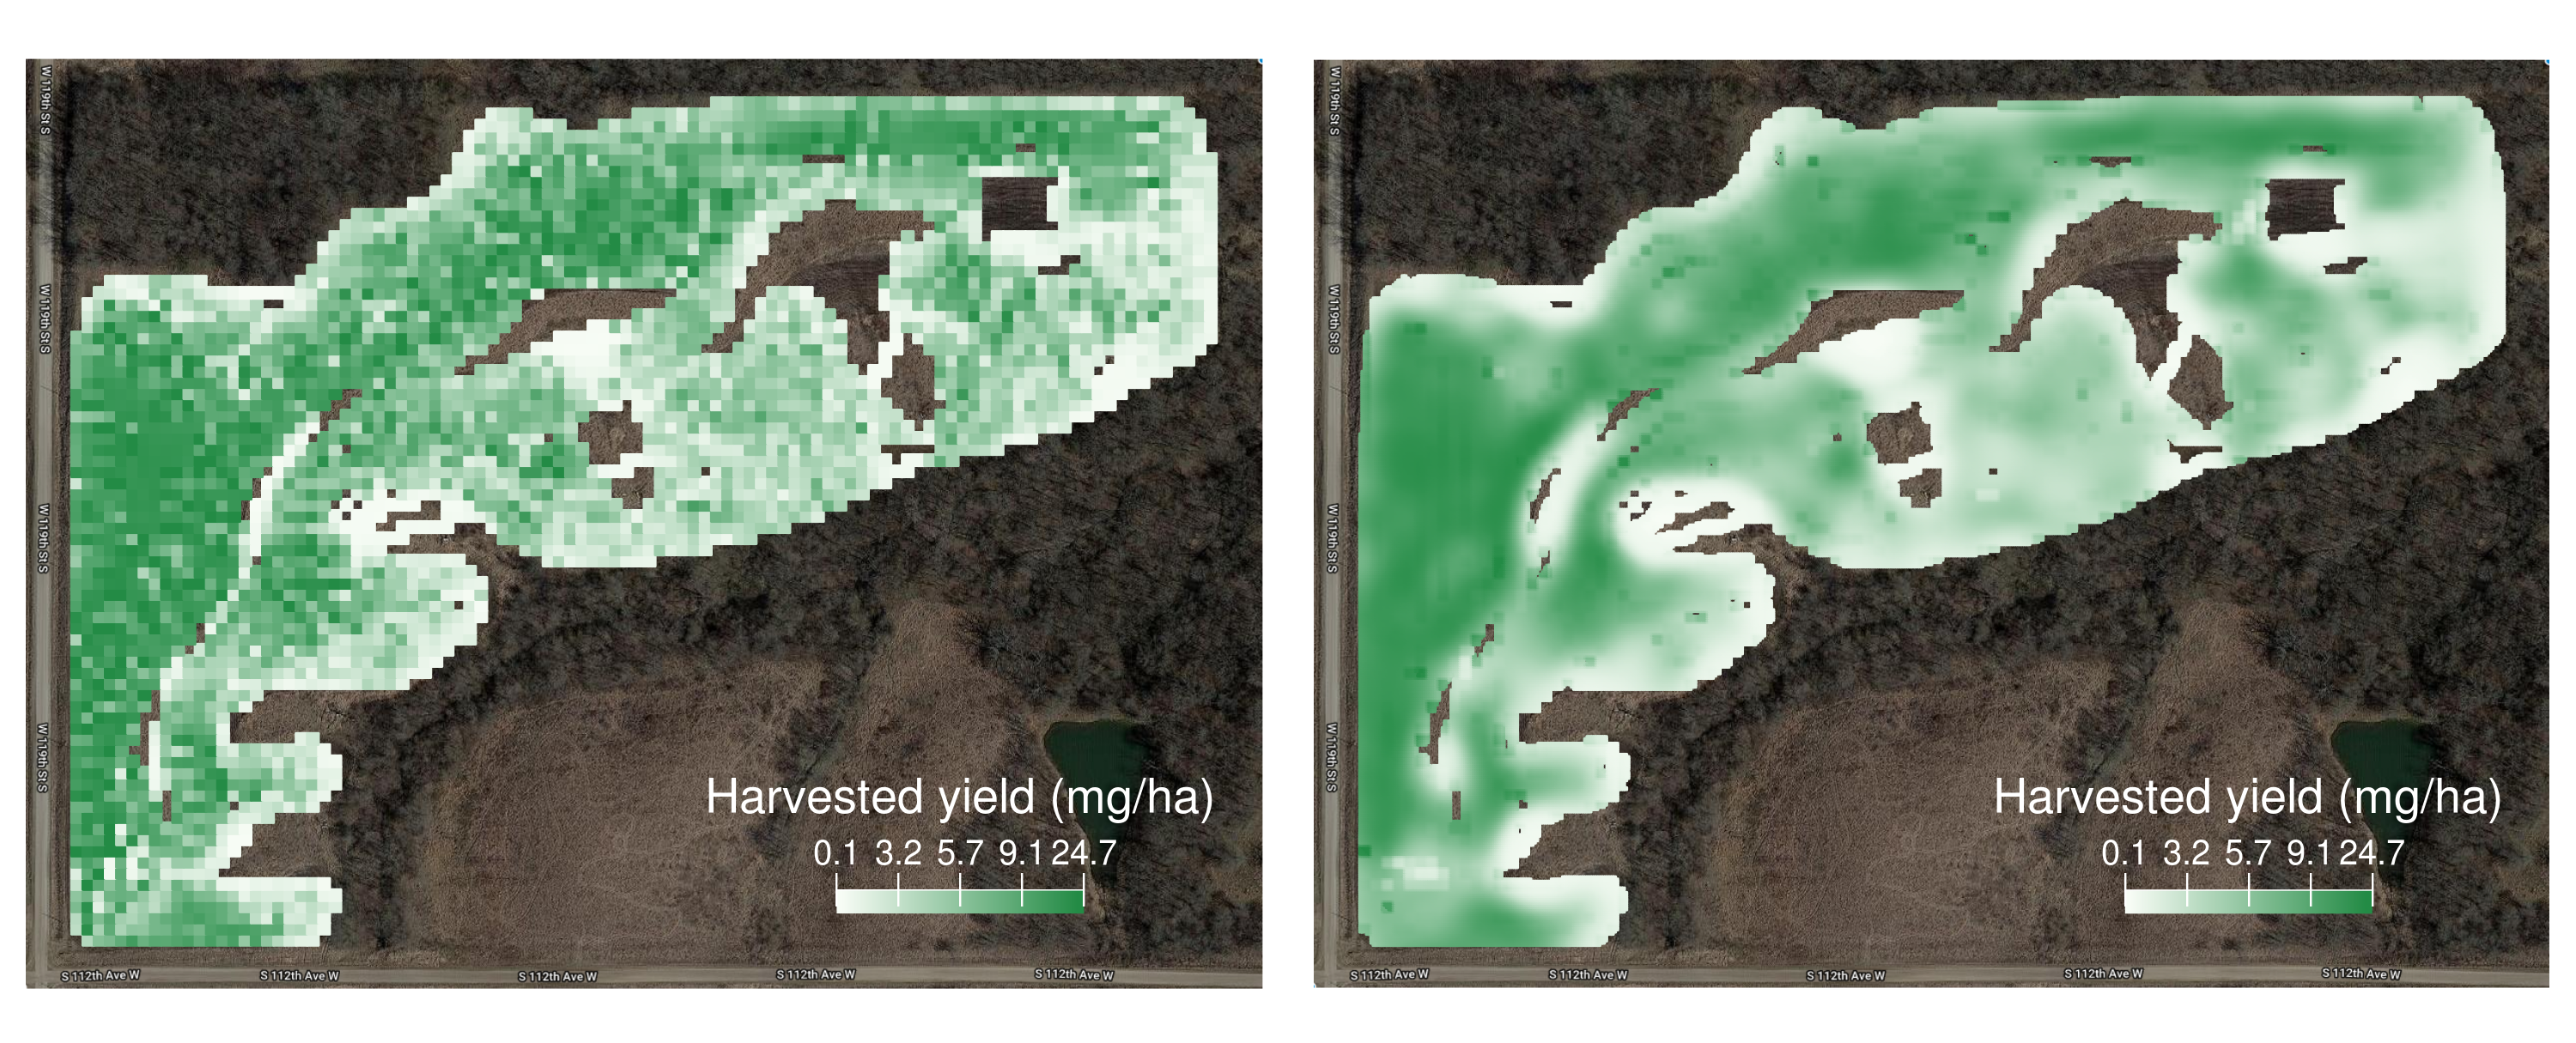
\includegraphics[width=0.49\textwidth]{basswood_2010_res5_1_agg_smoothed}
  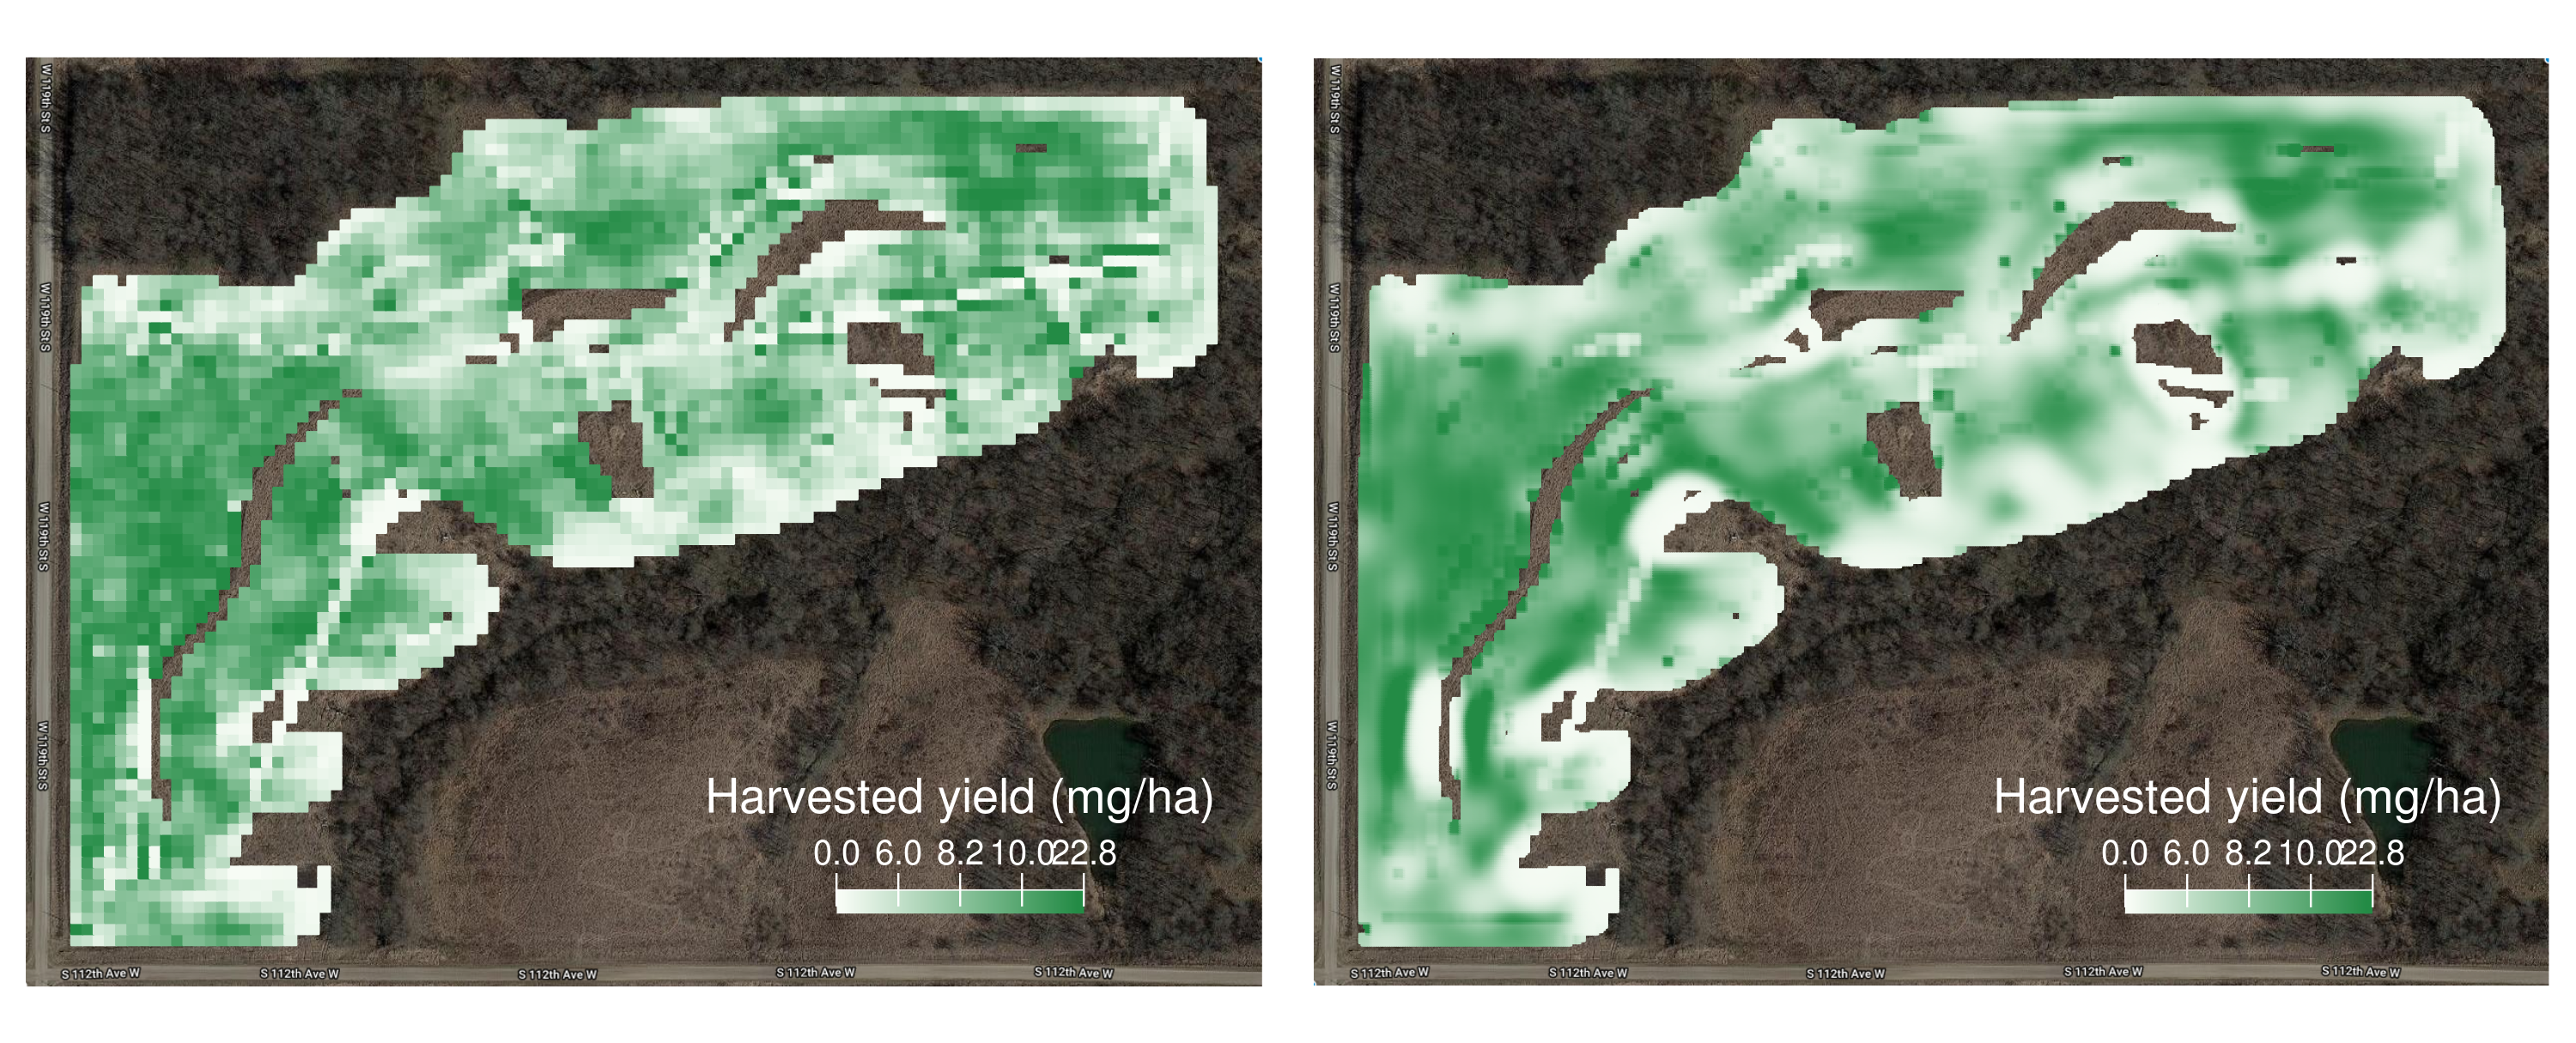
\includegraphics[width=0.49\textwidth]{basswood_2014_res5_1_agg_smoothed}
  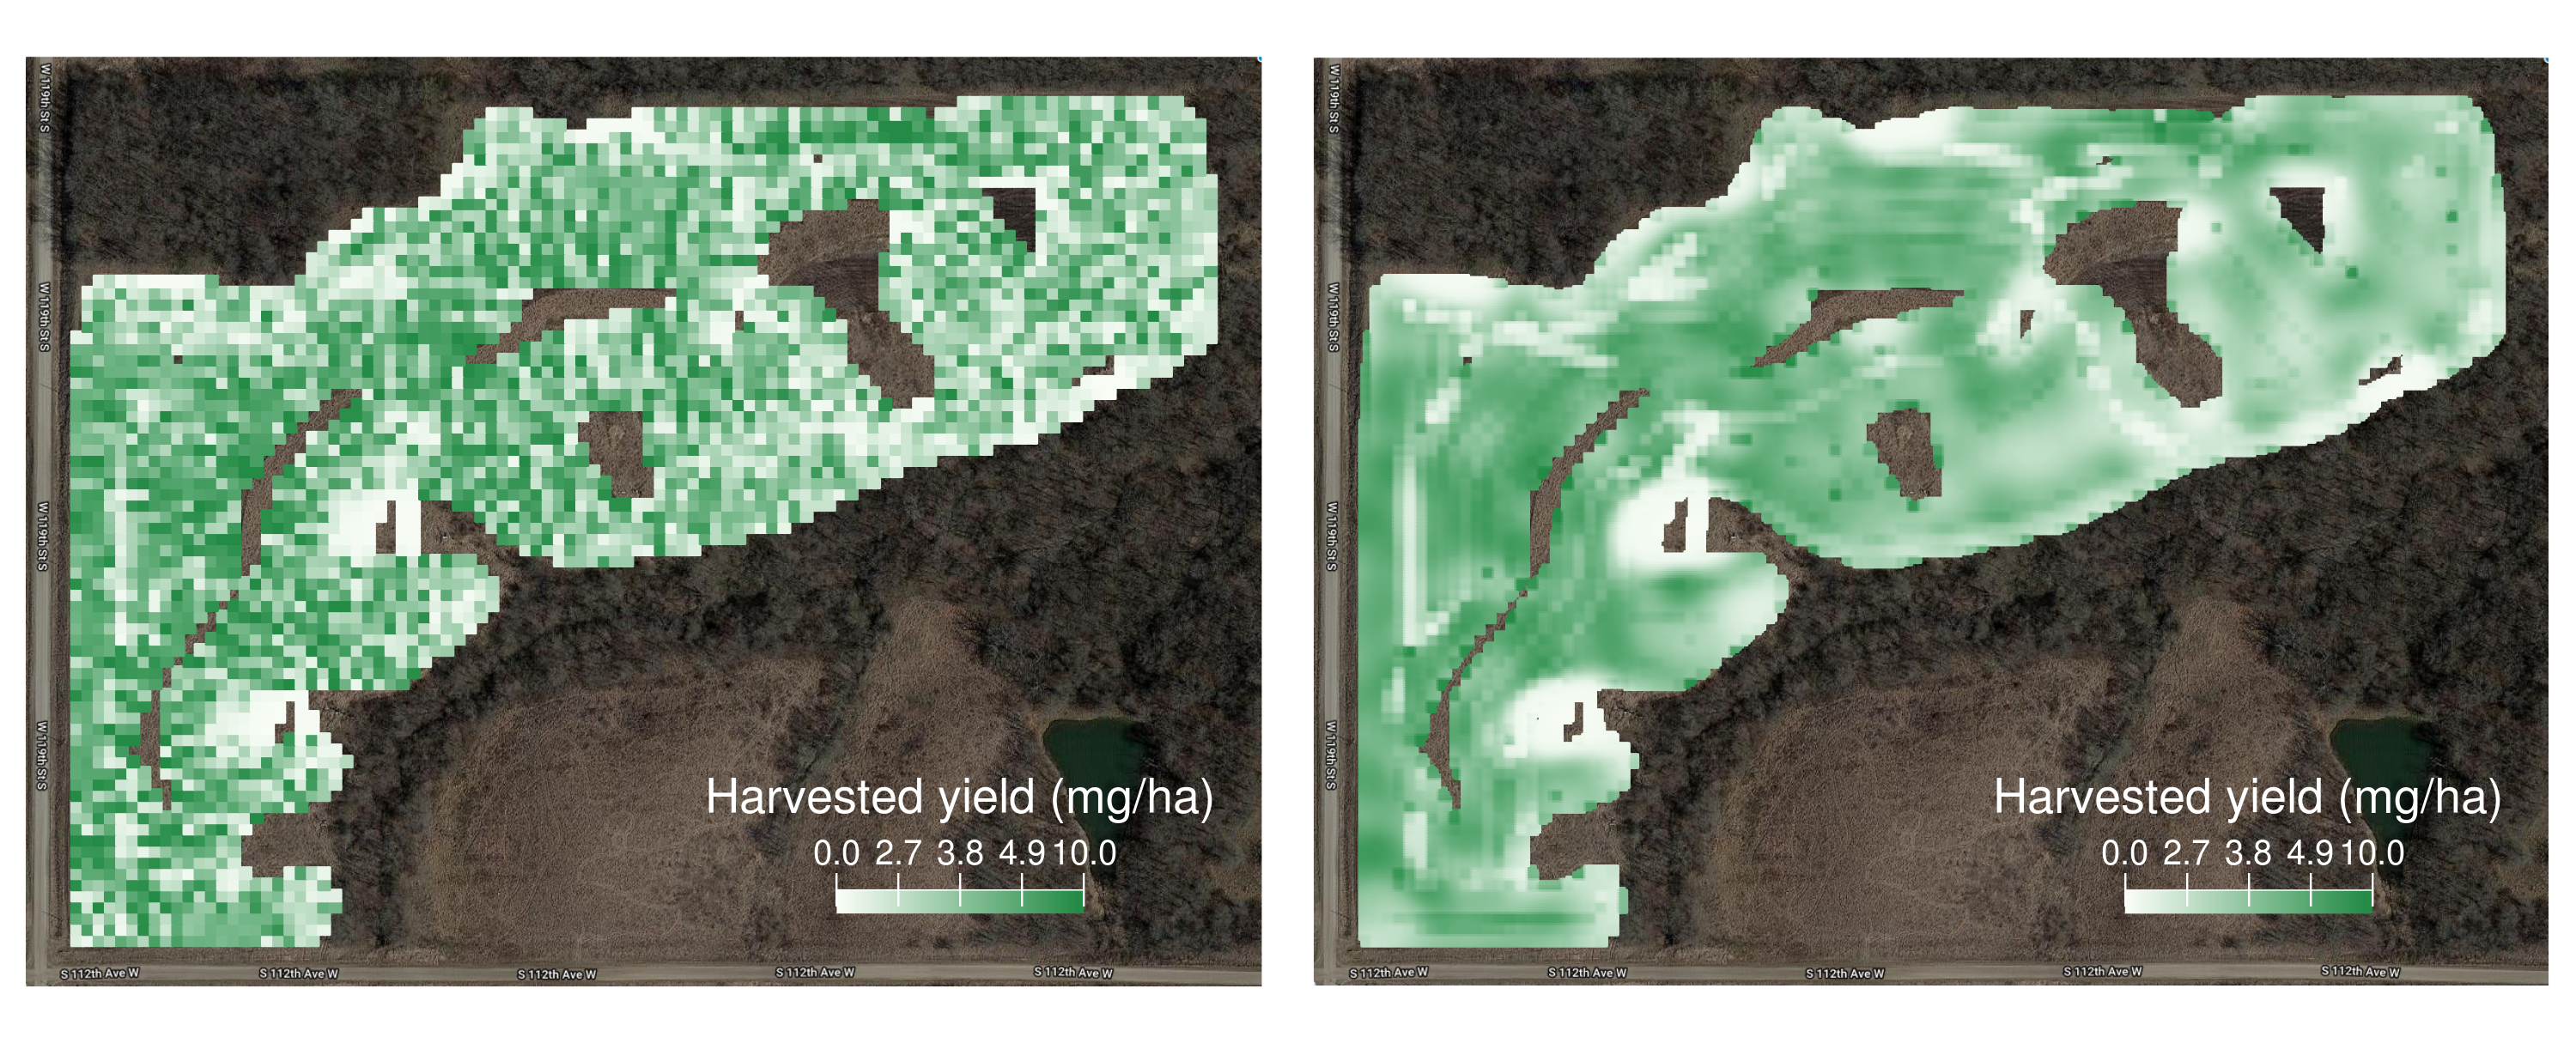
\includegraphics[width=0.49\textwidth]{basswood_2009_res5_1_agg_smoothed}
  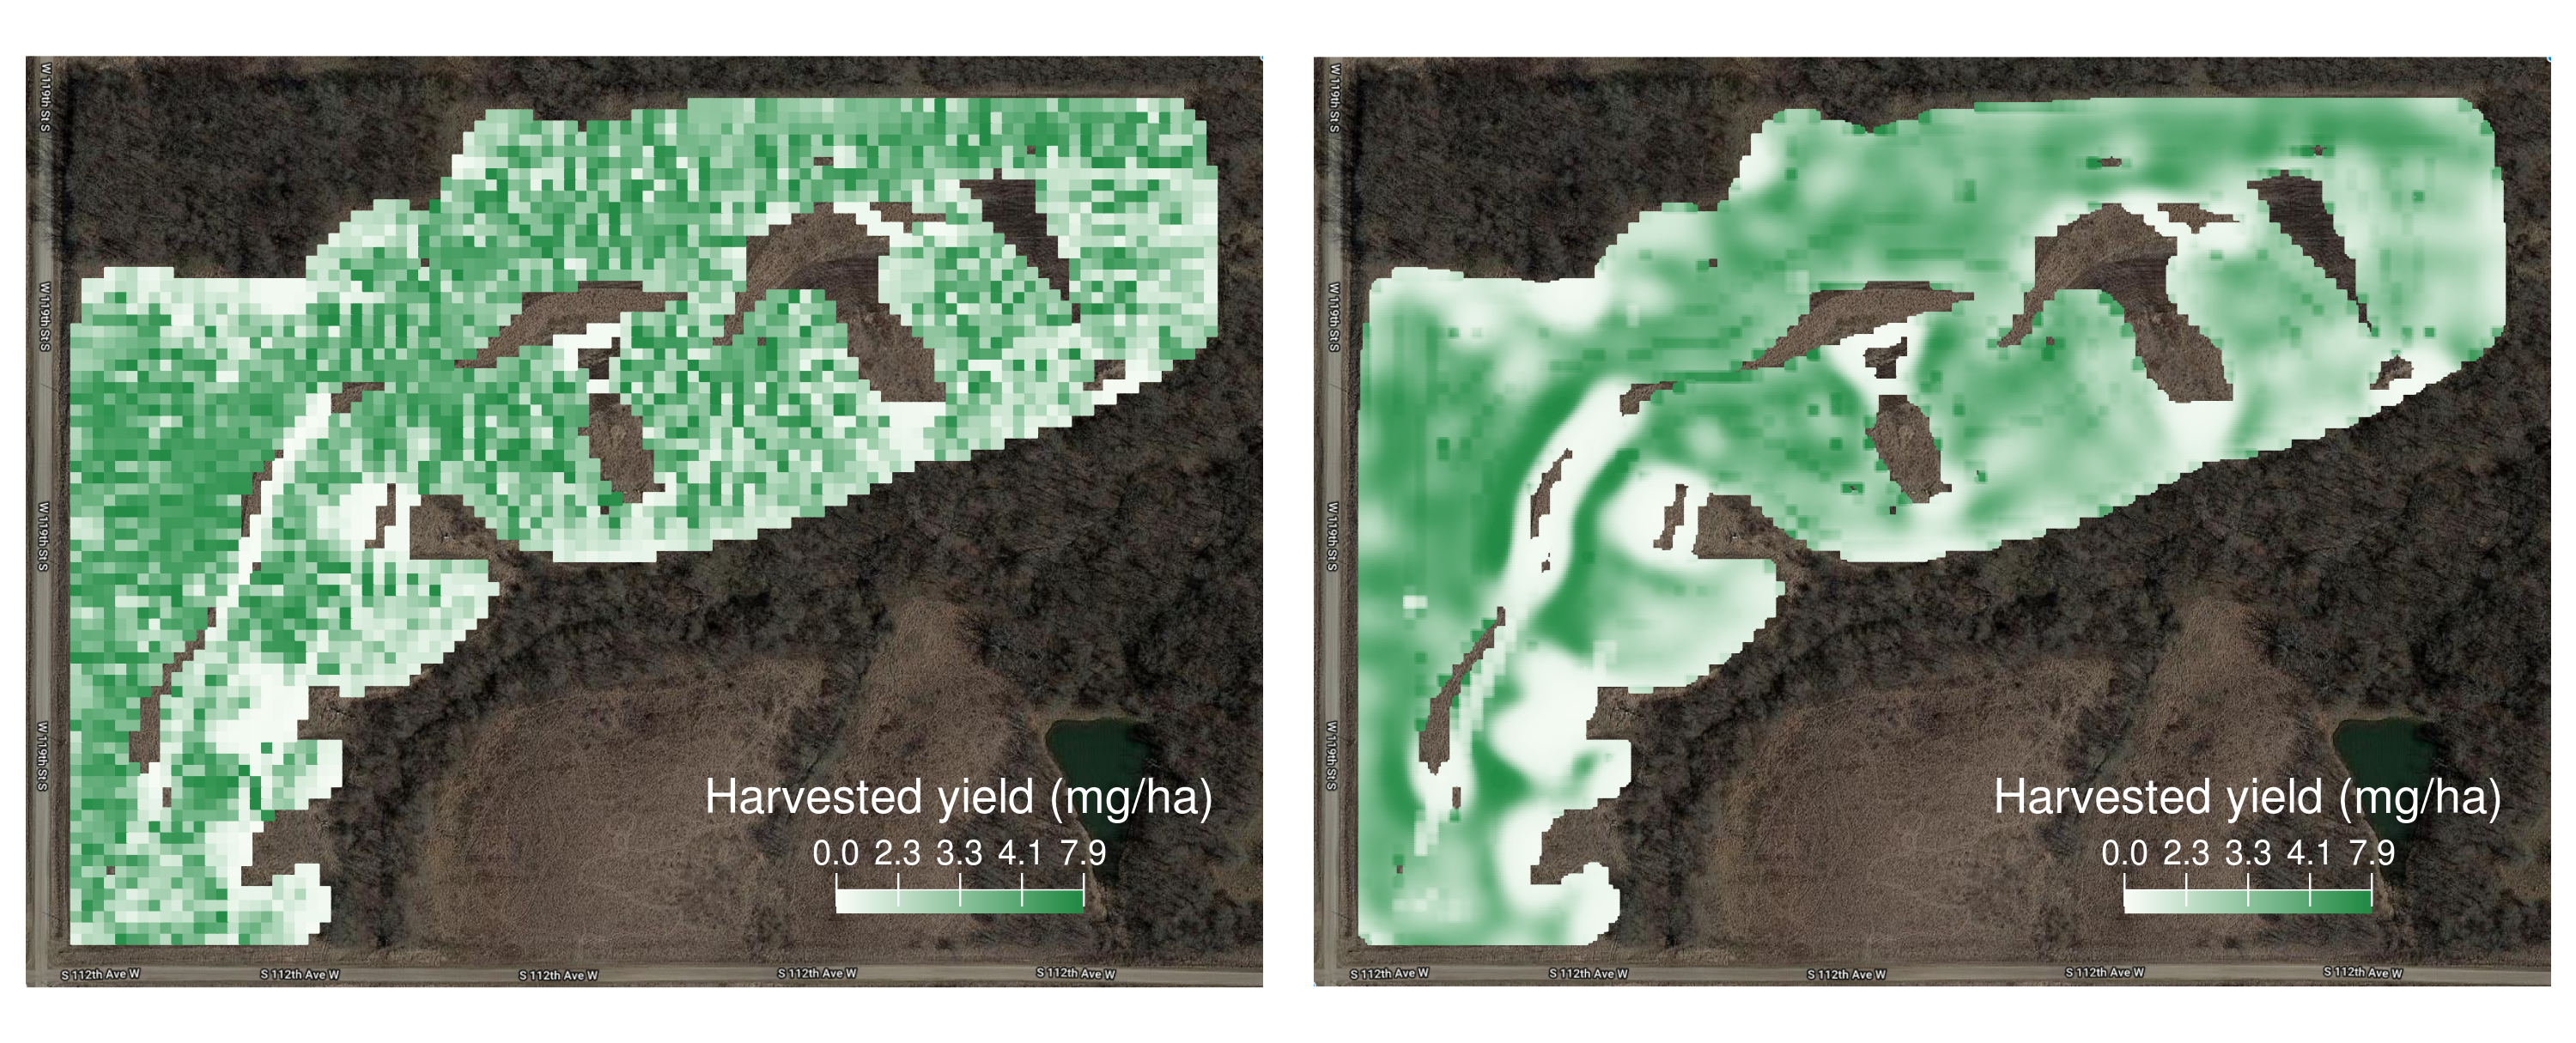
\includegraphics[width=0.49\textwidth]{basswood_2011_res5_1_agg_smoothed}
  \caption[Visualization of the algorithm output for one field across
  four different years]{Visualization of the harvested grain yield for
    Basswood in four different years. Maize in the top row, soybean in
    the bottom row. Aggregated yield in odd columns, smoothed yield in
    even columns. Although soybean data shows larger variability, as
    clearly displayed on the aggregated grid, the smooth map offer a
    clear visualization of the spatial trends. }
  \label{fig:basswood-history}
\end{figure}

%%% Local Variables:
%%% mode: latex
%%% TeX-master: "../thesis"
%%% End:

\chapter{Discussion}

\OUTLINE{Highlights about the algorithm} We have proposed an algorithm
for data processing and visualization that is designed for situations
where the destructive sampling scheme incorporates other non-trivial
features, namely time order and unequally-sized, irregularly-shaped,
and possibly overlapping areal observational units. Reproducing the
sampling process, the rules unpack the georeferenced coordinates,
recorded as points in a 2-dimensional space, into polygons that are
next tiled. The resulting geometries are aggregated using basic areal
units and apportioned assuming that the variable of interest follows a
uniform distribution at the local scale. The final output of the
processing rules is in the form of a regular tessellation of the
harvested area, equipped with both their associated observed and
smoothed yield; the output is meant for both data analysis and
visualization. As a byproduct, because the location of the pixels in
both the aggregation and smoothing grids can be chosen freely without
affecting the validity of the algorithm, spatial registration of the
output is readily available.

\OUTLINE{Comparison with previous work} To illustrate the main
characteristics of our procedure, we have presented a case study of
grain yield data processing and visualization. Whereas the previous
work in precision agriculture presents an almost unanimous preference
for extreme values detection and removal, with up to 32\% of the data
excluded \cite{Lyle2013}, our physically principled approach generates
a smooth visualization while retaining as much information as
collected. This improvement is partly explained by our reproducing of
the sampling scheme, but also by a twist on how the problem has been
traditionally framed: recognizing that local yield is a highly
volatile measurement unit due to scaling and error propagation, and
thus effectively shifting the baseline variable from yield to
mass. Also in contrast with previously proposed methodologies, most of
which require the map producer to set arbitrary thresholds, our
algorithm is autonomous. There are two main advantages associated with
this: (i) large amount of grain yield datasets can be processed
automatically, a relevant feature in the current times where data
collection has became accessible and widespread even at a small
farming scale; and (ii) the final outputs become more consistent
across different users, fields, and years.

% \OUTLINE{Our contribution (3) Implementation} Our contributions also
% includes an open-source implementation including both the processing
% rules as well as the visualization maps. The R package
% \texttt{yieldMap} provides tools to run this algorithm on the dataset
% used for the case study, which is provided along with the package as
% well, or simply on custom data. Besides providing some flexbility in
% terms of visualization options, it exploits parallelization when
% computing the smoothed yield via the Gaussian Process.

When doing exact inference for a Gaussian Process, smoothing requires
the inversion of a square matrix with size equal to the number of
observations in the aggregation step, which in this case study is
3,738 pixels. Unless resorting to approximate interpolation methods,
significant time is expected to be consumed for this purpose. As a
palliative, our implementation optionally divides the prediction space
into smaller subsets to be computed in parallel. Although there is no
direct gain in the matrix inversion time, it provides with some
marginal improvements as out prediction space is large with more than
90,000 pixels.

\OUTLINE{Future research: assumptions} Future improvements of this
algorithm could come from three perspectives: assumptions,
visualization, and computations. One of the main assumptions is that,
at a local scale, the random variable of interest follows a uniform
distribution. Although this is a reasonable idealization for the case
study given the small area of the observational units relative to the
rate of change of the underlying process, applications for
highly-distanced observations or rapidly-changing underlying processes
may require the extension to a different distribution
(e.g. exponential decay from the centroids of the polygons to its
boundaries). Yield monitors may record additional variables that are
currently not exploited by our algorithm, which could be enhanced for
example by smoothing via universal kriging with automatic relevance
determination for feature selection.

\OUTLINE{Future research: visualization} To improve visualizations,
the smooth map could profit from better display techniques to signal
the contrast between low and high valued areas (e.g. contour lines,
spatial clustering techniques). In the specific case of grain yield
maps, we still observe that some of the well-known sources of yield
data error transpire through the algorithm. Some of these can be
treated previously to running the algorithm, for example the time lag
effect, the harvester fill mode error, and position errors as
described in \cite{Blackmore1999}.

\OUTLINE{Future research: computation} On the computational side, the
case study suggests that the most time consuming steps are smoothing
and tiling, respectively. The former could be reduced by resourcing to
approximation methods for Gaussian Process spatial interpolation
\citep{Shi2007,Cressie2008,Katzfuss2011,Nguyen2012,Nguyen2014},
approximate linear algebra routines, or a more efficient interpolation
technique. Although the intrisic sequential nature of the sampling
scheme limits the potential of parallelization in the tiling step,
some performance improvements could be potentially achieved by
subviding the spatial domain into disjoint blocks that should after be
accordingly recoupled (divide and conquer). Alternatively, the bitmap
matrix of \cite{Han1997} could be revisited as an approximation to our
polygon approach. These gains could turn the current work into a near
real-time algorithm.


%%% Local Variables:
%%% mode: latex
%%% TeX-master: "../thesis"
%%% End:


% \include{reference/biblio}
\renewcommand{\bibname}{\centerline{BIBLIOGRAPHY}}
\unappendixtitle
\interlinepenalty=300
\newpage
\phantomsection
\begingroup
    \setlength{\bibsep}{13.2pt}
  \linespread{1}\selectfont
\addcontentsline{toc}{chapter}{BIBLIOGRAPHY}
\bibliography{reference/references}
\unappendixtitle
\endgroup

%%% Local Variables:
%%% mode: latex
%%% TeX-master: "../thesis"
%%% End:


% Appendix1 file from standard thesis template

\appendixtitle 
\appendix

%% Use the following two lines for single appendix
\unappendixtitle
\singleappendixtitle

\chapter{ADDITIONAL MATERIAL} 

\TODO{Some of these figures repeat in Figure 2. Find a better strategy for this.}

\begin{figure}
    \centering
    \begin{minipage}{0.49\textwidth}
        \centering
        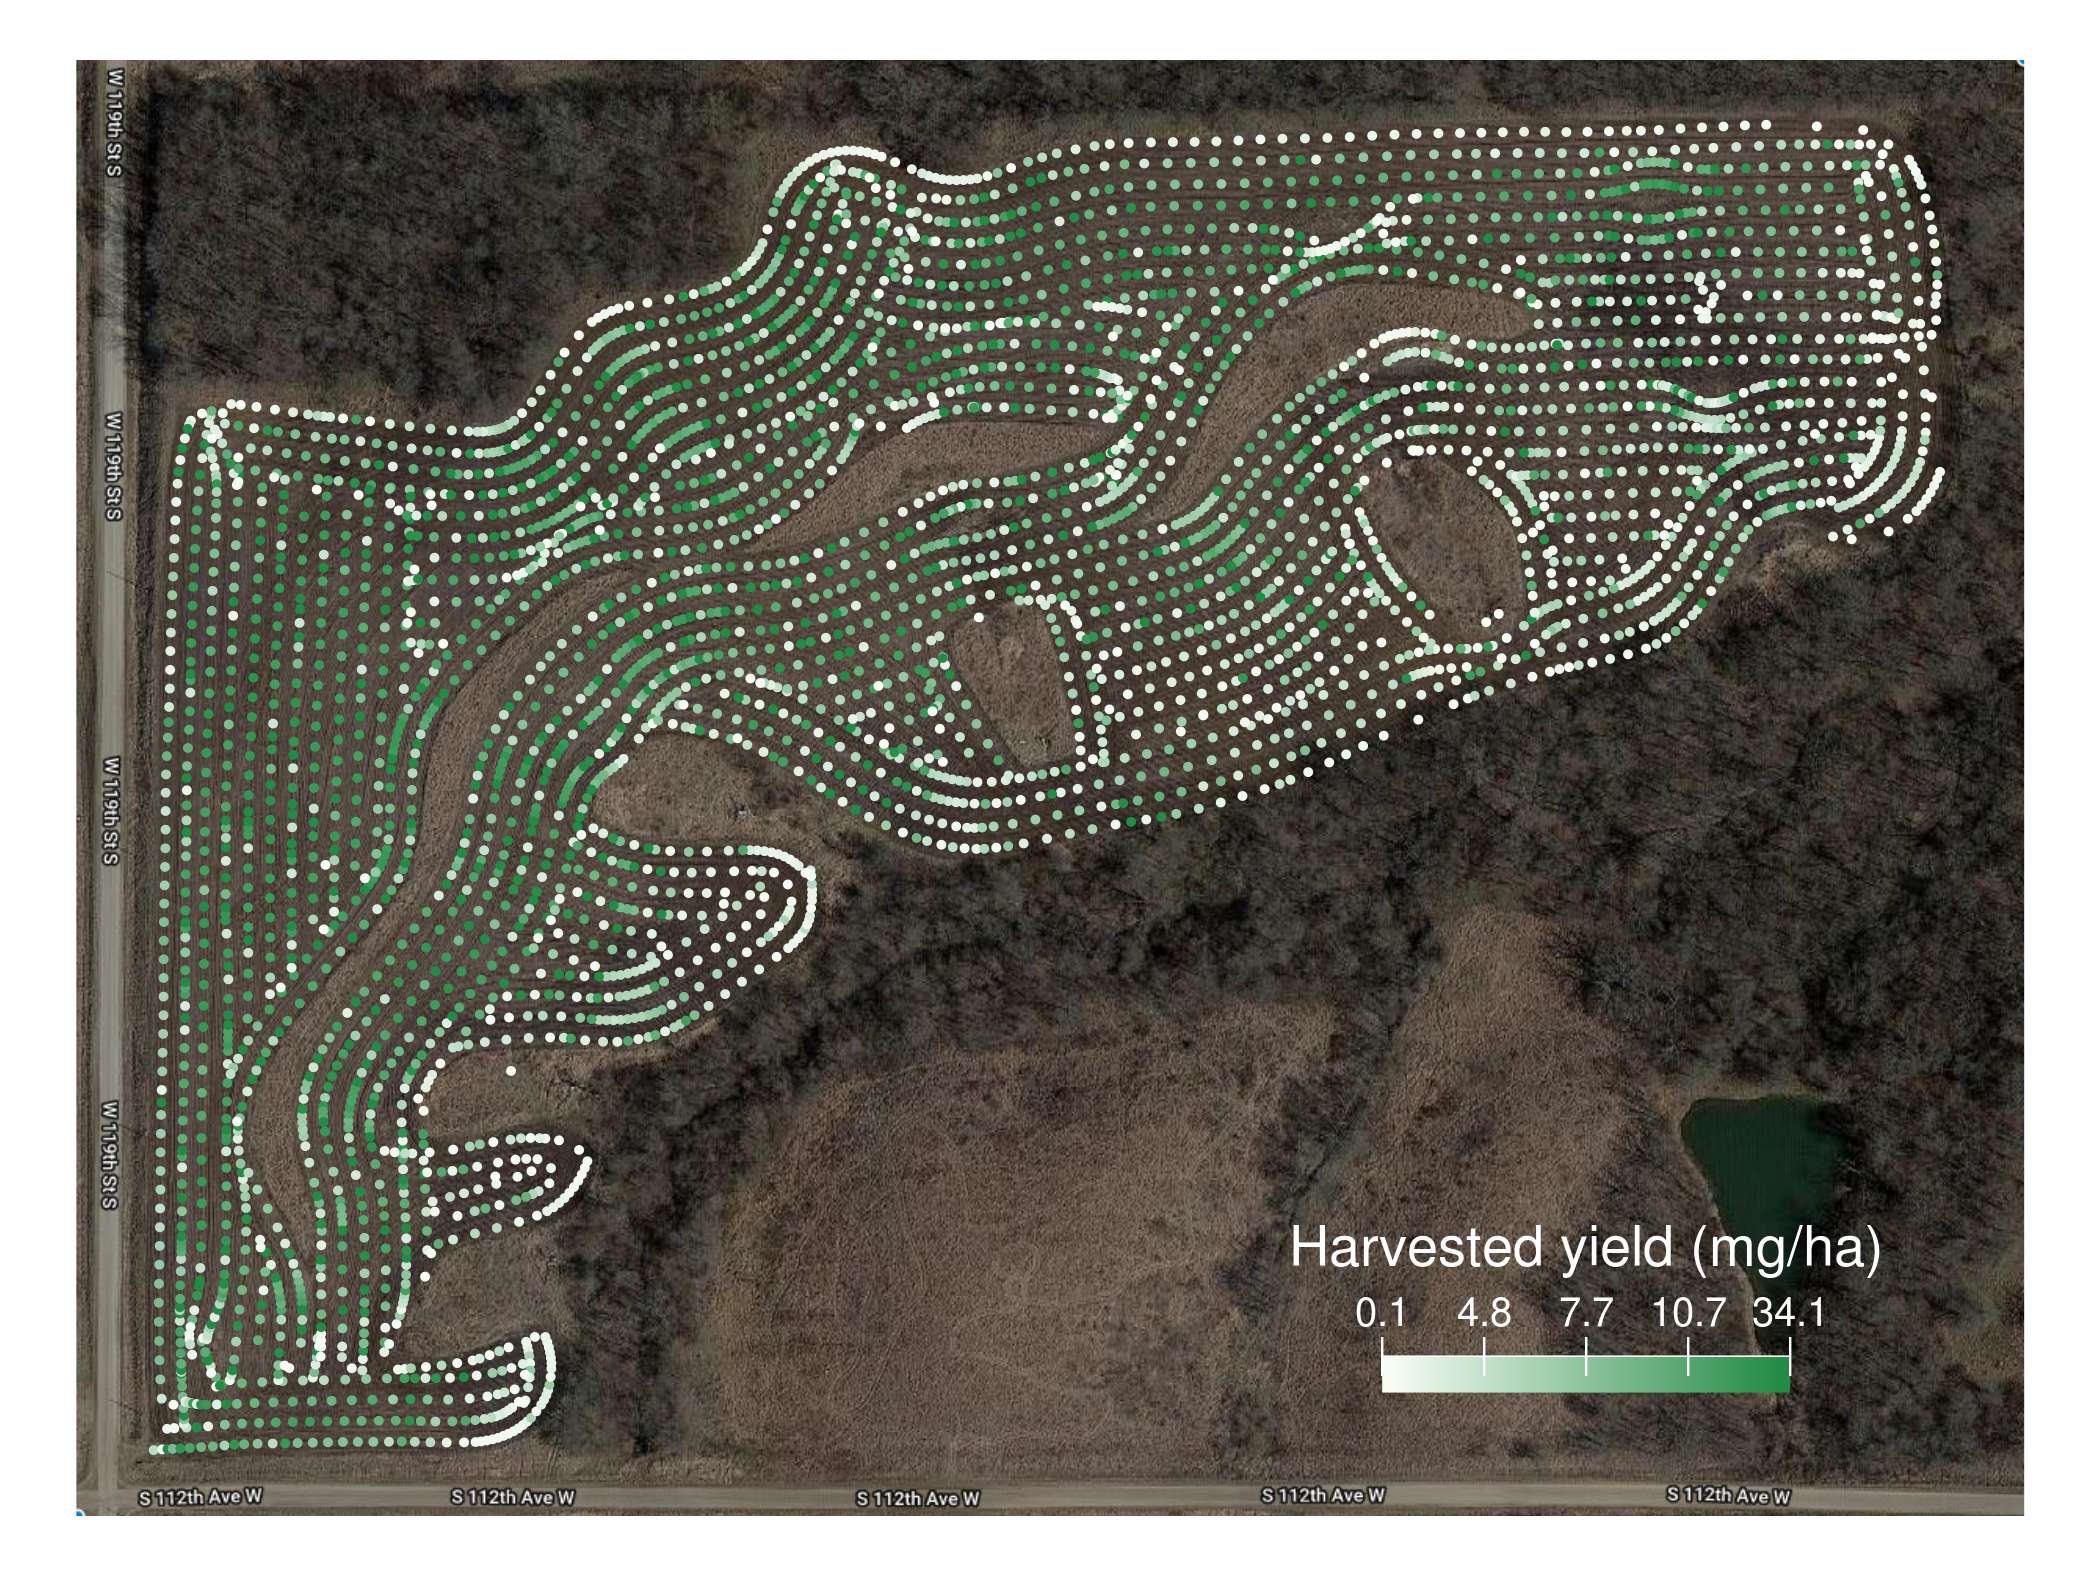
\includegraphics[width=0.75\textwidth]{appendix/basswood_2012_res5_1_points_vehicle}
        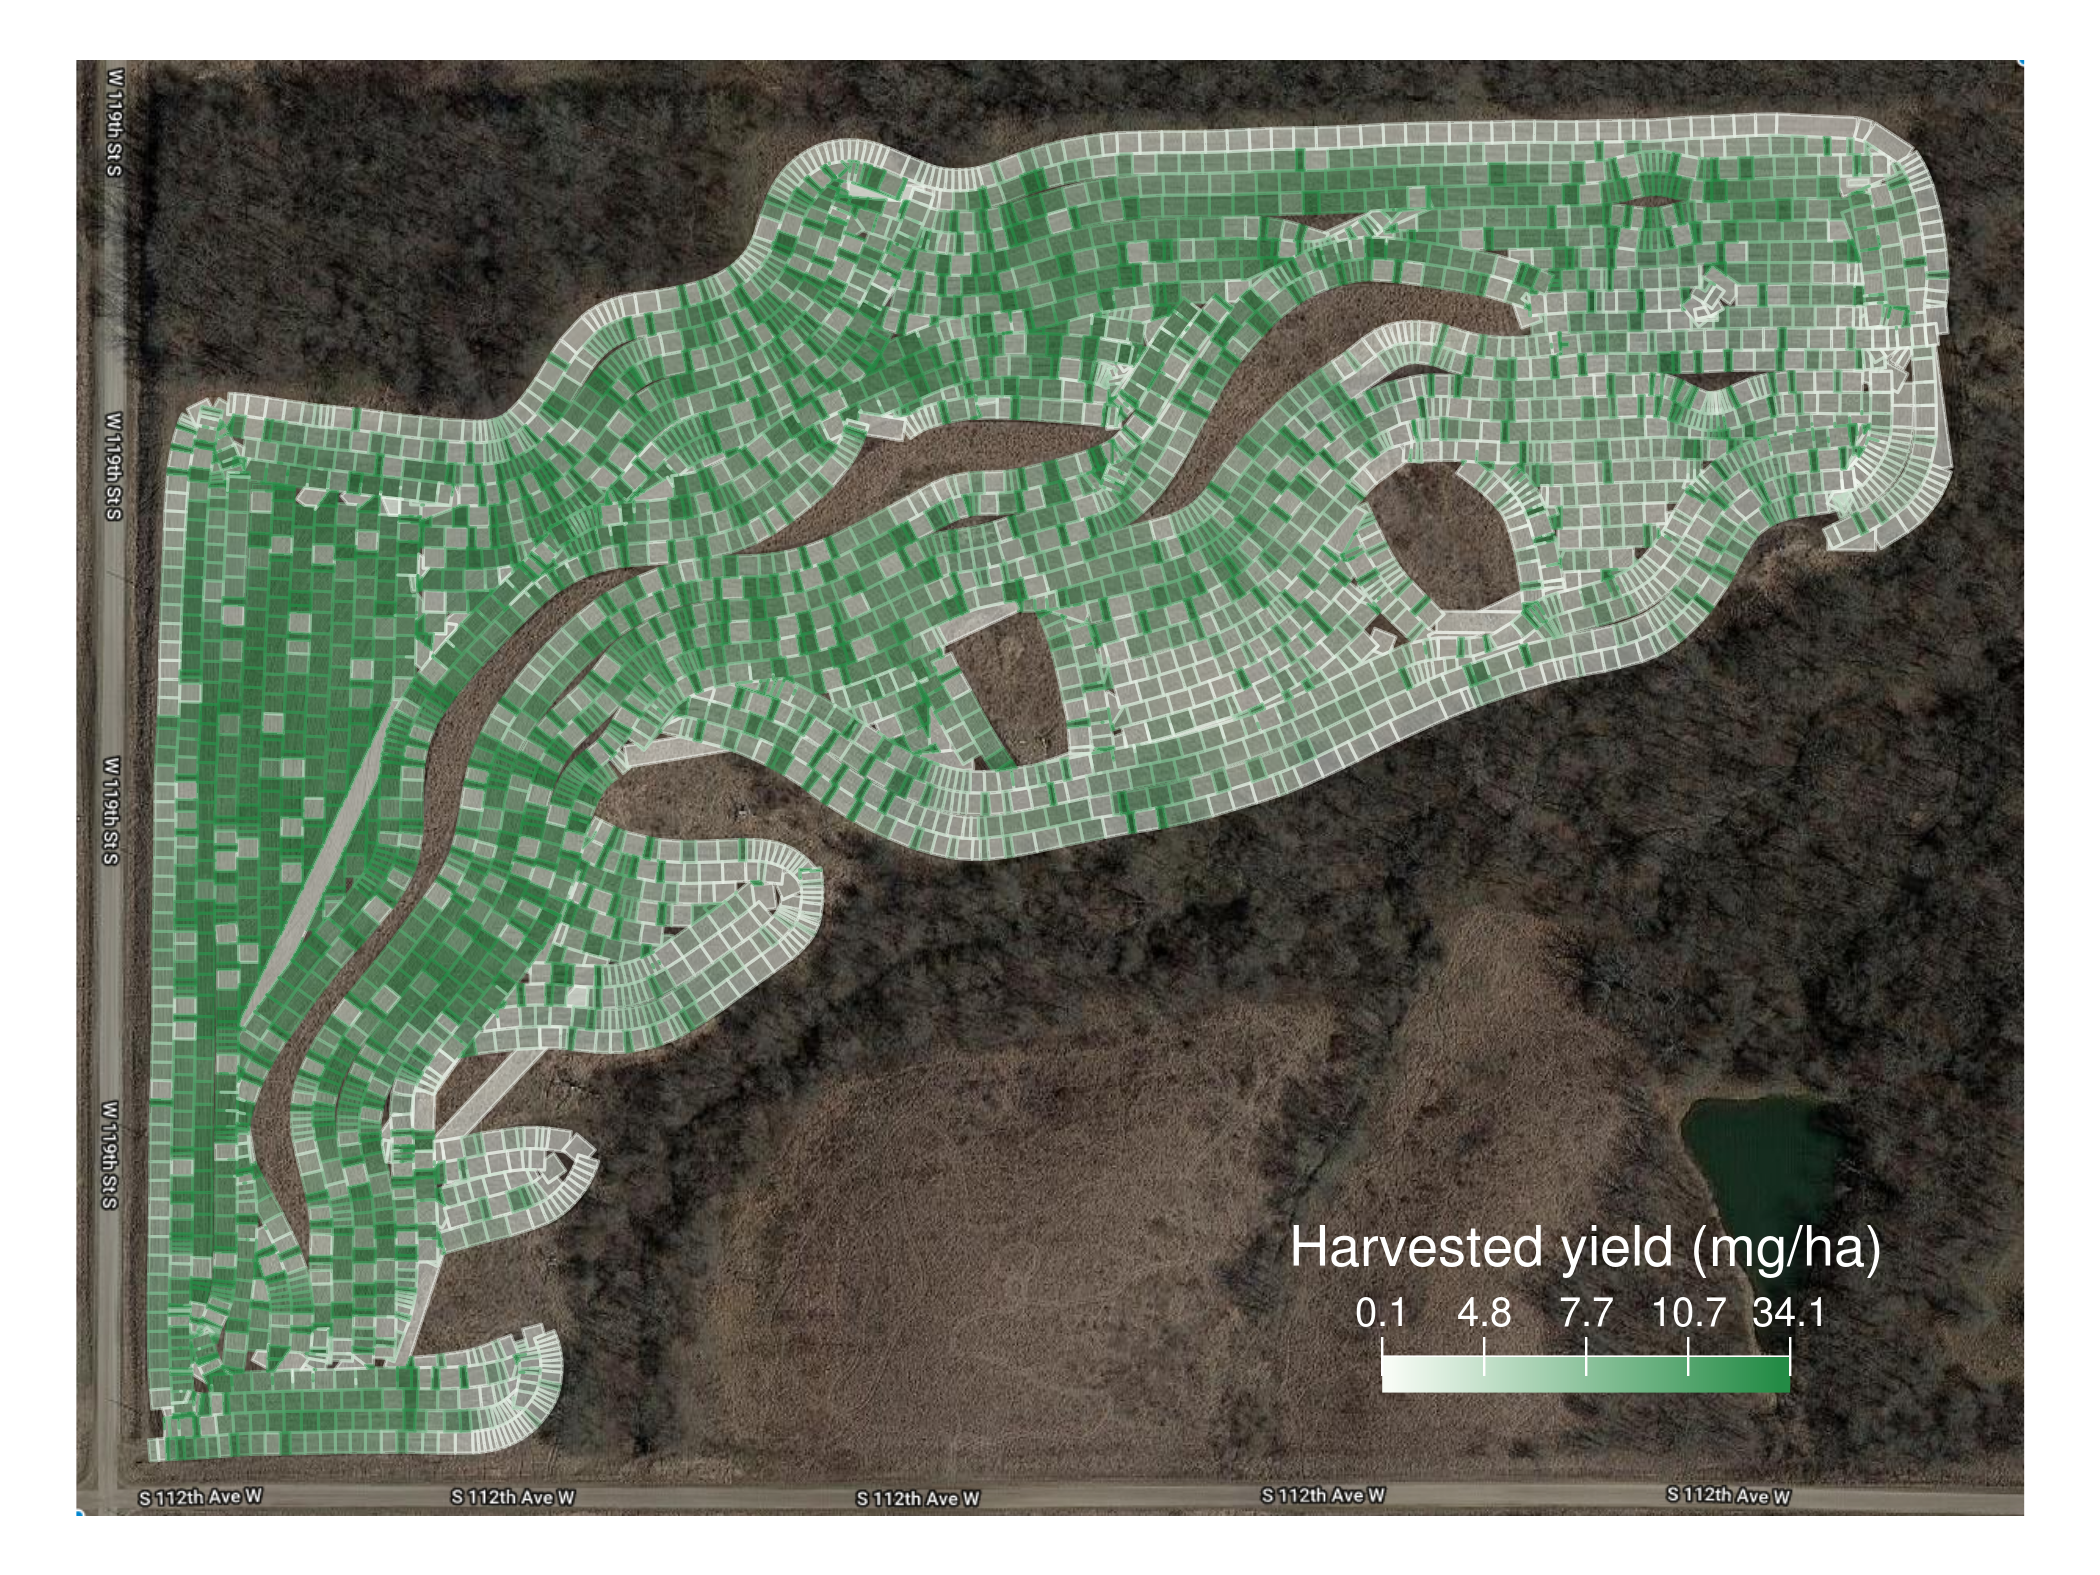
\includegraphics[width=0.75\textwidth]{appendix/basswood_2012_res5_1_reshaped}
        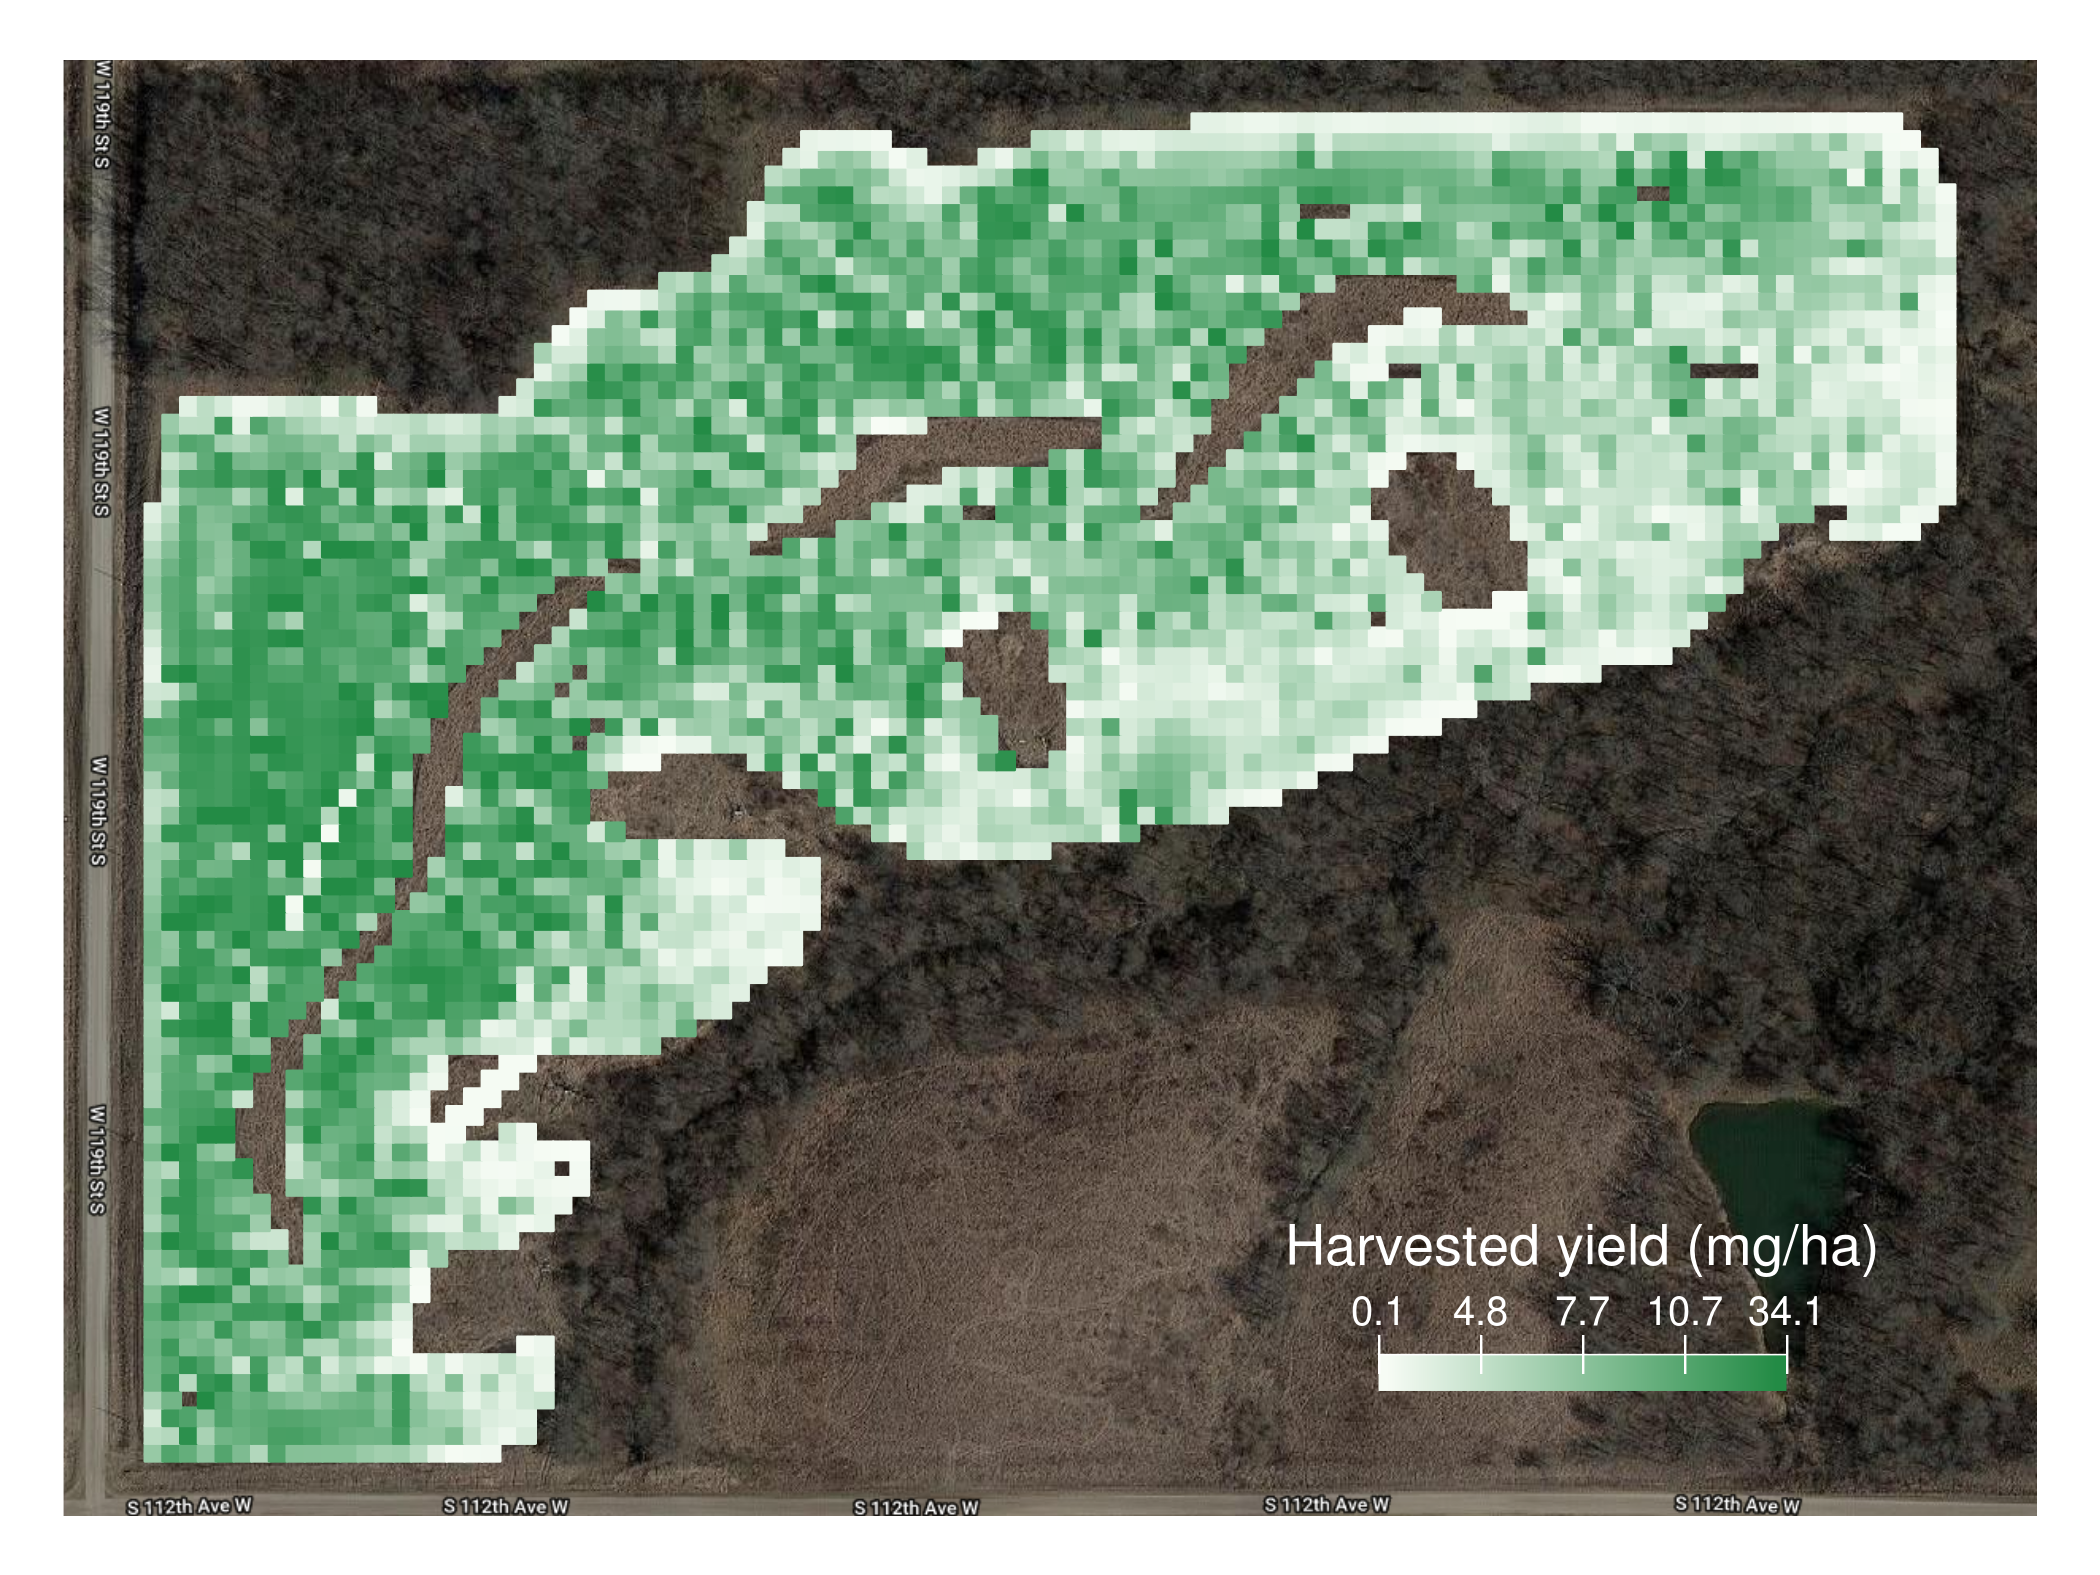
\includegraphics[width=0.75\textwidth]{appendix/basswood_2012_res5_1_aggregated}
    \end{minipage}\hfill
    \begin{minipage}{0.49\textwidth}
        \centering
        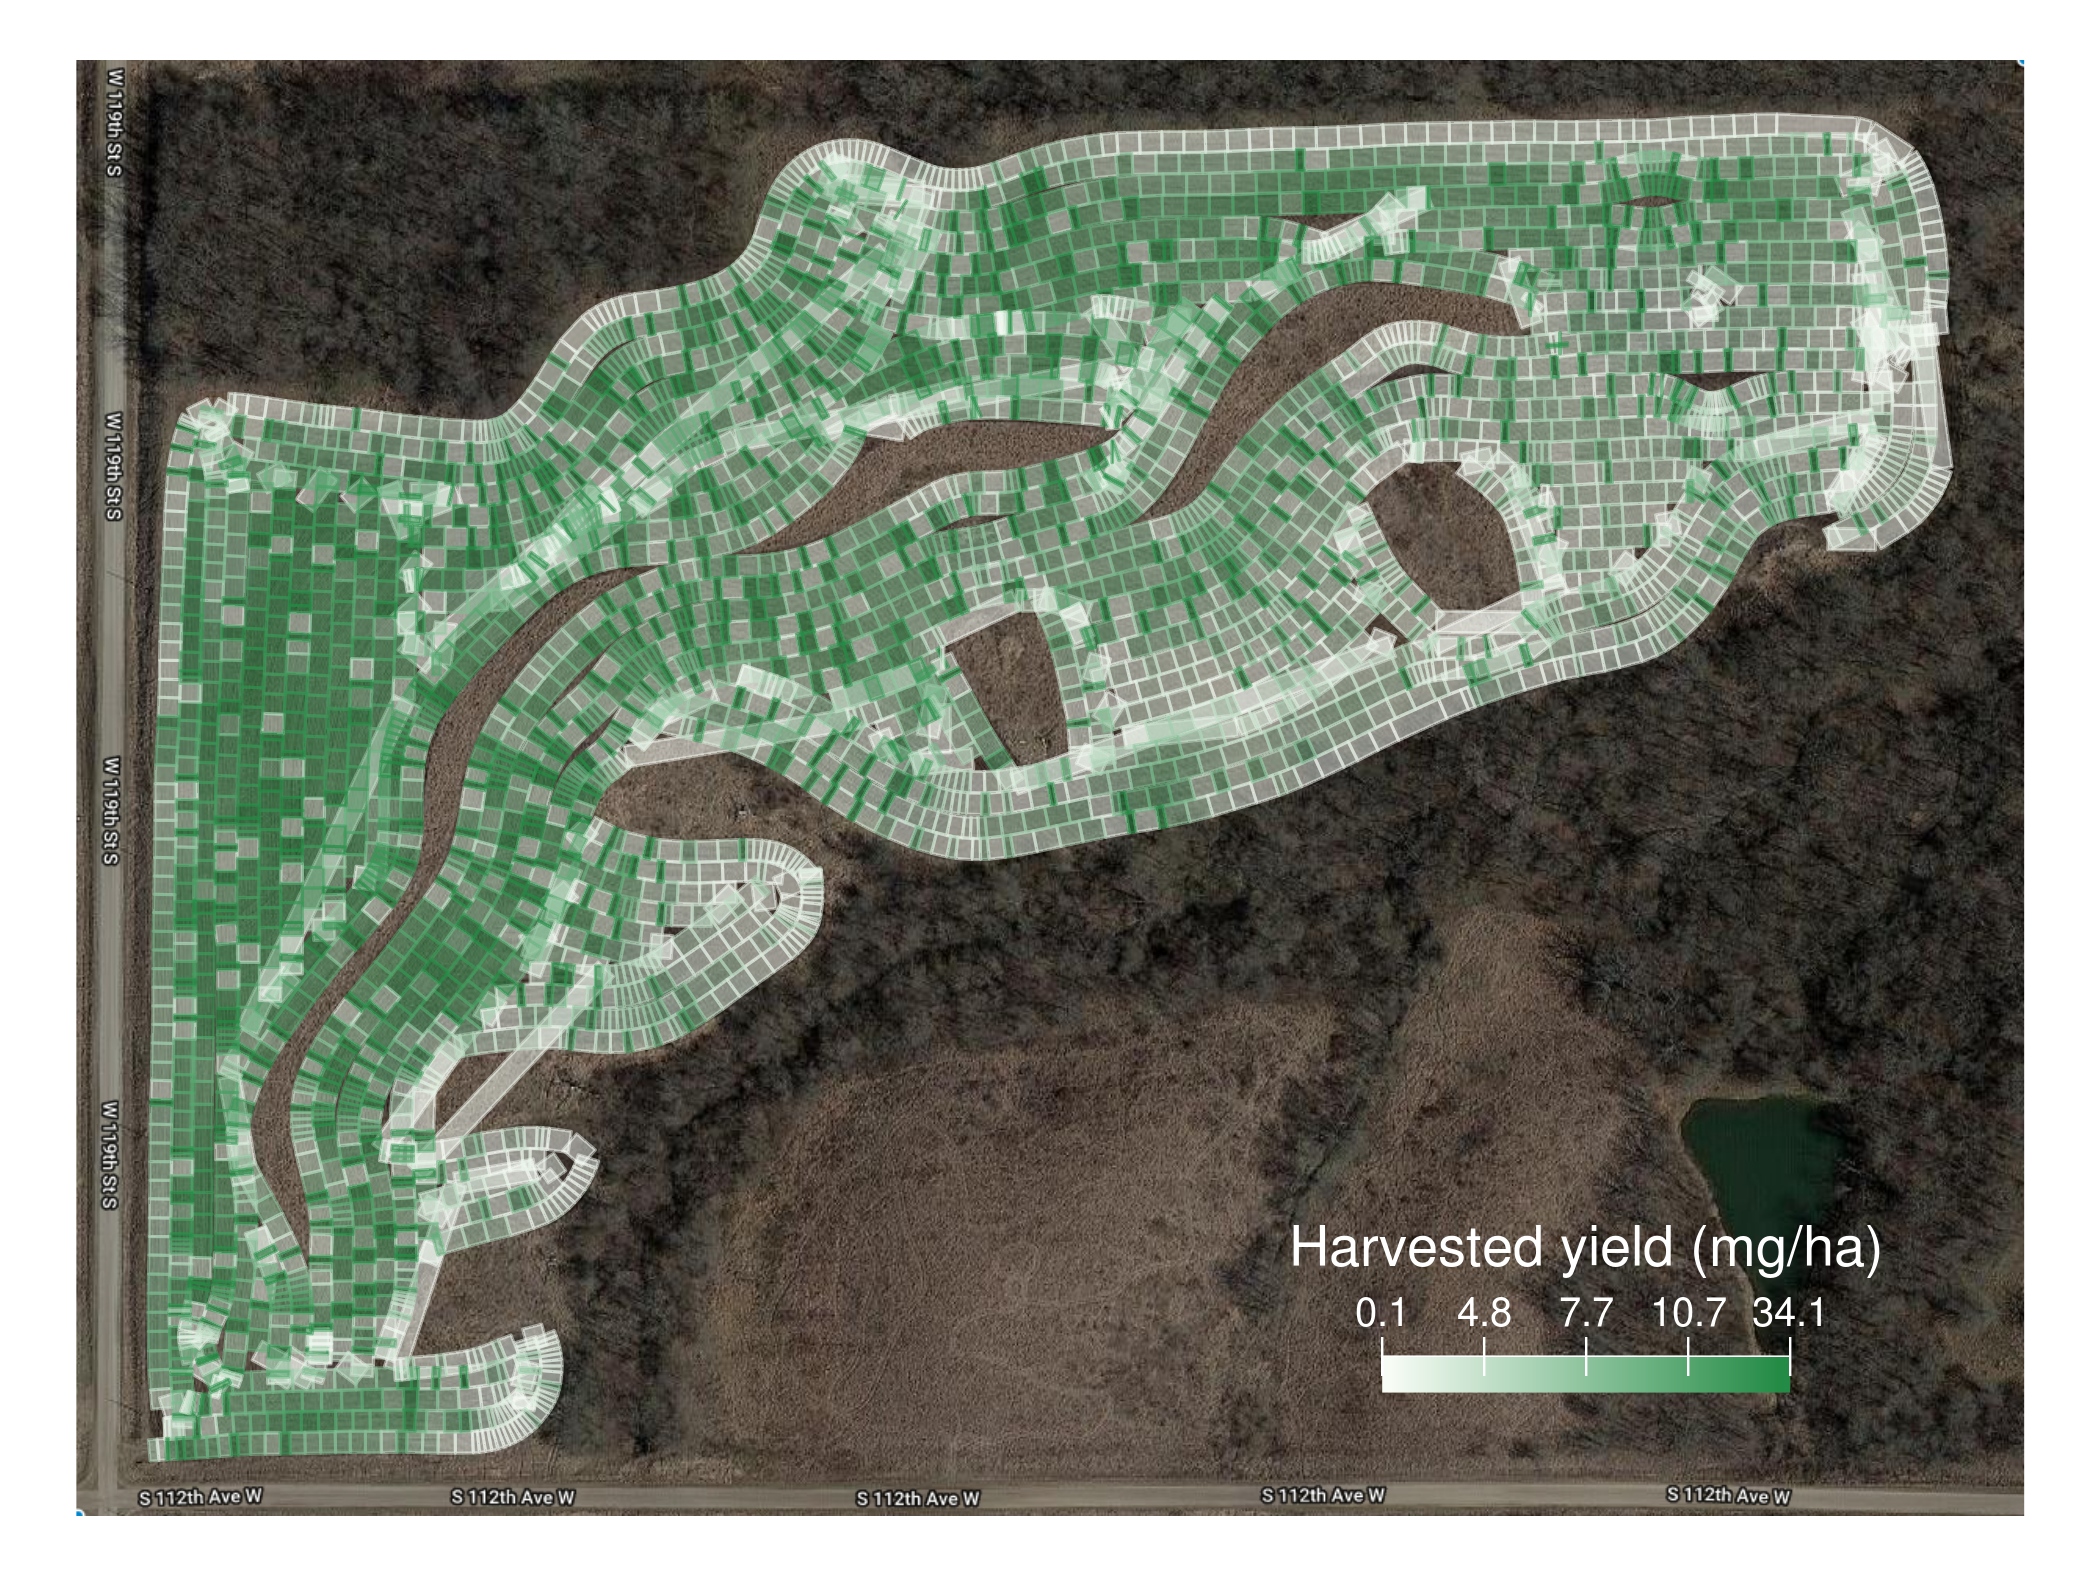
\includegraphics[width=0.75\textwidth]{appendix/basswood_2012_res5_1_polygons_vehicle}
        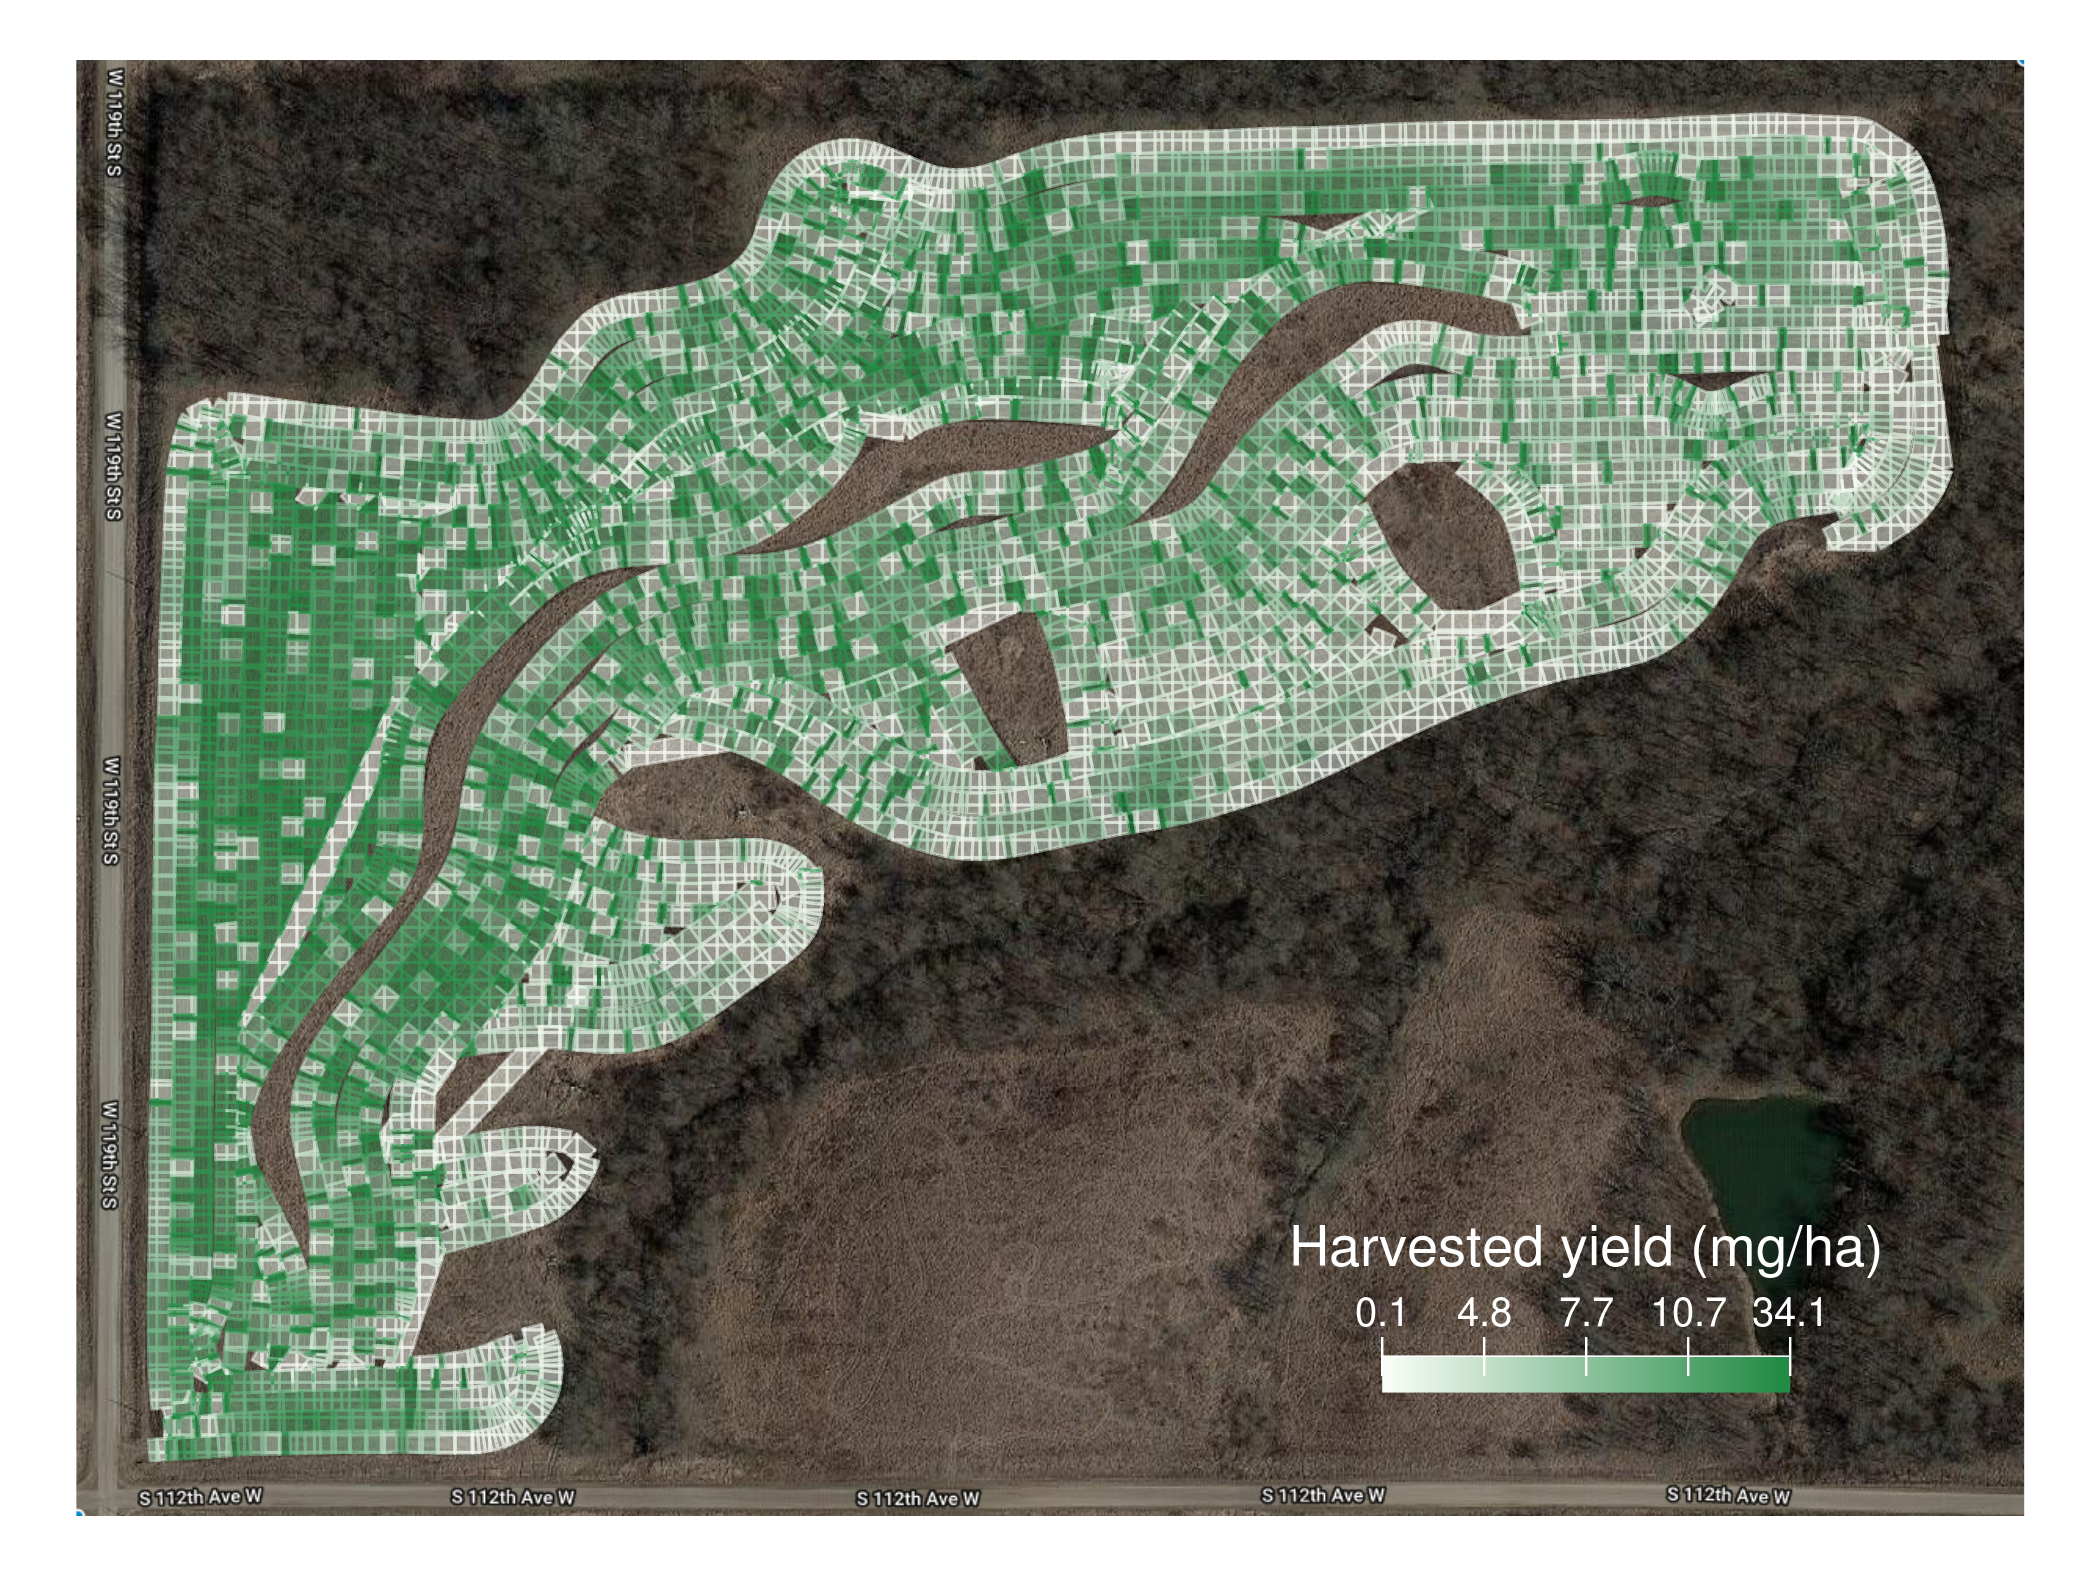
\includegraphics[width=0.75\textwidth]{appendix/basswood_2012_res5_1_chopped}
        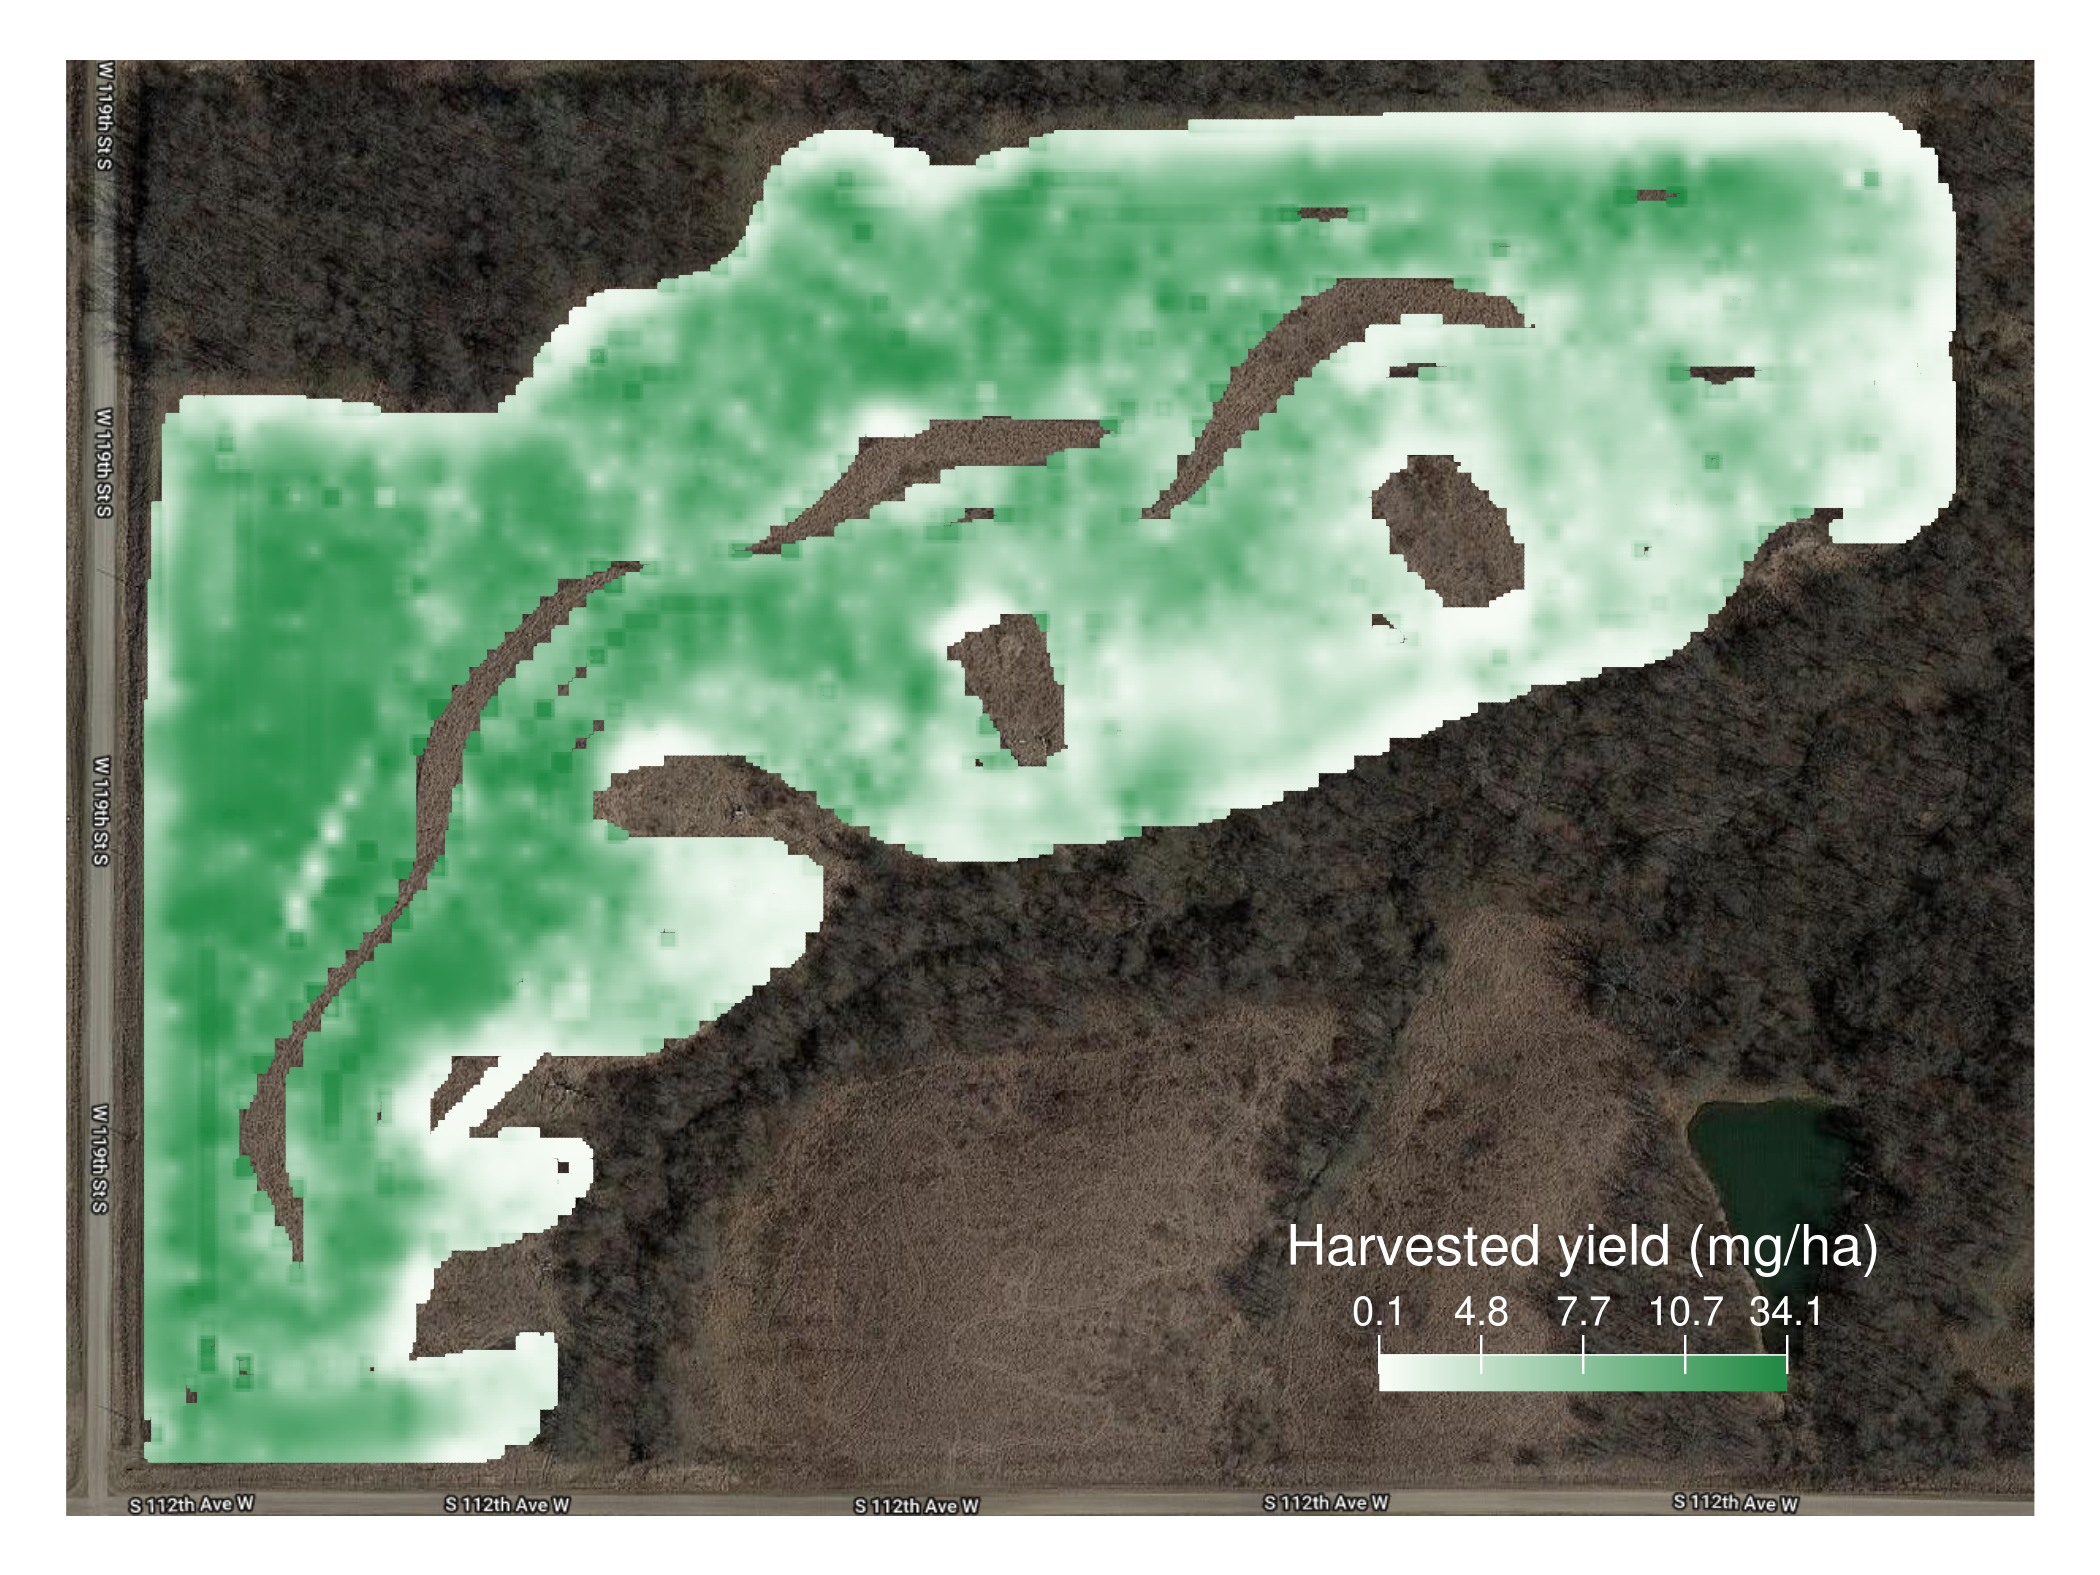
\includegraphics[width=0.75\textwidth]{appendix/basswood_2012_res5_1_smoothed}
    \end{minipage}
    \caption{Every step progression. Figures should be viewed from left to right. Brief explanation.}
    \label{fig:basswood2012-all-steps}
\end{figure}


%%% Local Variables:
%%% mode: latex
%%% TeX-master: "../thesis"
%%% End:


\end{document}

% IMPORTANT NOTES TABLE OF CONTENTS : TOPIC 1: If you need a page
% break follow the steps below step1 check before which chapter in the
% table of contents you want a page break step 2 go the folder
% "body". There open the chapter tex file that you noted needed page
% break in the table of contents..  step 3 insert
% \addtocontents{toc}{\protect\newpage} before the first line
% i.e. before the line \chapter{RESULTS}.

%%%%%%%%%%%%%%%%%%%%%%%%%%%%
% \def\@makechapterhead#1{%
% IN ORDER TO MAKE spacing changes in the title page got to the
% section in the isuthesis.cls file that starts with
% \long\def\maketitle{\begin{titlepage} and you can use options like
%   singlespace (less spacing) singlespacing (comparitively more
%   spacing almost like 2 spacing) onehalfspacing doublespacing (this
%   is more spacing than the singlespacing above ) more definitions on
%   spacing can be found by going through the class file

%   use \isucaption{} for all captions of figures and tables, where
%   the captions are not too long.

%   Use \isucaption[]{} with the square brackets for short caption of
%   figure or table that goes into the list of tables and list of
%   figures, and the curly brackets can have long captions which go
%   with the figure/ table.

%%%%%%   Using sub figures
% %%%   In preamble include : \usepackage{subfig}
%   \begin{figure}[htbp]
%     \centering \subfloat[first
%     caption.\label{fig:2a}]{\includegraphics[width=0.2\textwidth]{Images/dc5.jpg}}\hfill
%     \subfloat[second caption.\label{fig:2b}]
%     {\includegraphics[width=0.2\textwidth]{Images/dc5.jpg}}\hfill
%     \isucaption{Sub-figure test}
%     \label{fig:subfigure-test}
%   \end{figure}

%   Subfloat reference: Fig \ref{fig:2a}

%   Figure reference: Fig \ref{fig:subfigure-test}
	

%%% Local Variables:
%%% mode: latex
%%% TeX-master: t
%%% End:
